\chapter{Data-Aware Accelerator Design}
\label{chap:dda}

As discussed in \autoref{chap:background:intro}, any convolution accelerator can
be reduced into it's dataflow and hardware implementation choices. Based on the
dataflow exploration approach in \cite{dnn_df_overrated_v1} dataflows are
explorable through the nested loop structure that makes up a convolution
layer introduced in \autoref{chap:background:intro}.
The design space dimensions of dataflows is comprised of:
\begin{itemize}
    % \item Loop ordering of the nested loops structure
    \item Loop unroll targets (which loops are unrolled and which are not) 
    \item Loop unroll factors for the loop unroll targets
    \item Mapping of loops to an accelerators spatial axis of which there are 2
\end{itemize}

Ideally dataflow design space exploration should be hardware implementation
agnostic. We can enumerate the size of the design space by examining the scope
of the afformentioned design space dimensions. Beginning with the choice of loop
unroll targets. One can choose to unroll only one loop or all loops with
varying unroll factors. Unrolling loops exposes opportunities for parallelism
when executing unrolled loops on an accelerator. Therefore the number of
possible combinations of loop unroll targets is
$\sum\limits_{l=1}^{6}\binom{6}{l}$ with a total of $6!$ possible orderings for
said loops. The space of possible loop unroll axis mappings is $\binom{l}{\min(2,
l)}$ depending on the chosen number of loops $l$ unrolled. The space of possible
unroll factors is then dictated by the upperbounds of the indexes in the loop
representation $max(F).max(C).max(Y).max(X).max(KY).max(KX)$ and the upperbound
of the available processing engines $Count_{pe}$. Some combination of upper
bounds are very unlikely to occur in real networks which limits the size of the
design space for loop unroll factors. However, when considering the
mapping of unrolled loops to an accelerator's spatial axis, the choice of unroll
factors becomes more complicated. When two loops are unrolled in the same
spatial axis, the effective unroll factor for each one of them may change when
processing a layer with a different convolution layer configuration than the one
assumed when unrolling the loops. For example, consider the following situation.
For a convolution layer with kernel size 3x3 and channel count 32, if the kernel
loops are unrolled fully with an unroll factor of 9, and the channel loops are
unrolled partially with an unroll factor of 4, and they were both mapped to the
same spatial axis, then the total number of processing engines allocated to that
spatial axis would be 36. After allocating those PEs, if we attempt to execute a
different convolution layer with a different configuration, for example, a 1x1
convolution layer with 32 channels, the allocated PEs would be underutilized because
the effective channel unroll factor would be 36 instead of 4 in the original
configuration.

In this chapter we will first prune the dataflow design space dimensions in
\autoref{chap:dda:dataflow_dse:pruning} by determining the apprioriate
loop unroll targets and loop unroll factors using insights acquired from
\ac{CIGAR} a convolutional network analysis tool discussed in
\autoref{chap:dda:dataflow_dse:pruning:cigar}. Then, given the complexity of
exploring loop unroll factors and loop axis mapping, an automated accelerator
Template optimizer TEMPO introduced in \autoref{chap:dataflow_dse:exploring} is
used to explore the the afformentioned design space dimensions to produce
utilization optimized accelerator template configurations. 

\section{Pruning the dataflow design space with CIGAR}
\label{chap:dda:dataflow_dse:pruning}

\subsection{CIGAR: The ConvolutIon statIstics GAtherer}
\label{chap:dda:dataflow_dse:pruning:cigar}

\subsubsection{Algorithm}
\label{chap:dda:dataflow_dse:pruning:cigar:algo}

Psudocode for \ac{CIGAR}'s algorithm is presented in algorithm
\ref{alg:cigar_algo}. In algorithm \ref{alg:cigar_algo}, \ac{CIGAR} begins by
calling Collect\_Library\_Statistics after acquiring a dictionary of pytorch
models $modell_{dict}$. Collect\_Library\_Statistics then instantiates an empty
$model^{stats}_{dict}$ to be populated with model layer statistics . It then
instantiates a collector object that acts as a container for collected model
statistics. For each model, a new input image tensor is created based on the
requirements of the model being analyzed. If no special transformations are
required a default image tensor configuration is used where the width and the
height dimension of the image is set 224x224 with 3 RGB channels. After an image
tensor is created, Attach\_Collection\_Hooks is called to attach the collector
object's extract\_stats callback function or hook on each Conv2D layer present
in the model's layers. Attach\_Collection\_Hooks returns an array to each
attached hook to be later detached once the model under inspection is processed.
An illustration of this process is given in \autoref{fig:cigar_extraction}.

\begin{figure}
    \centering
    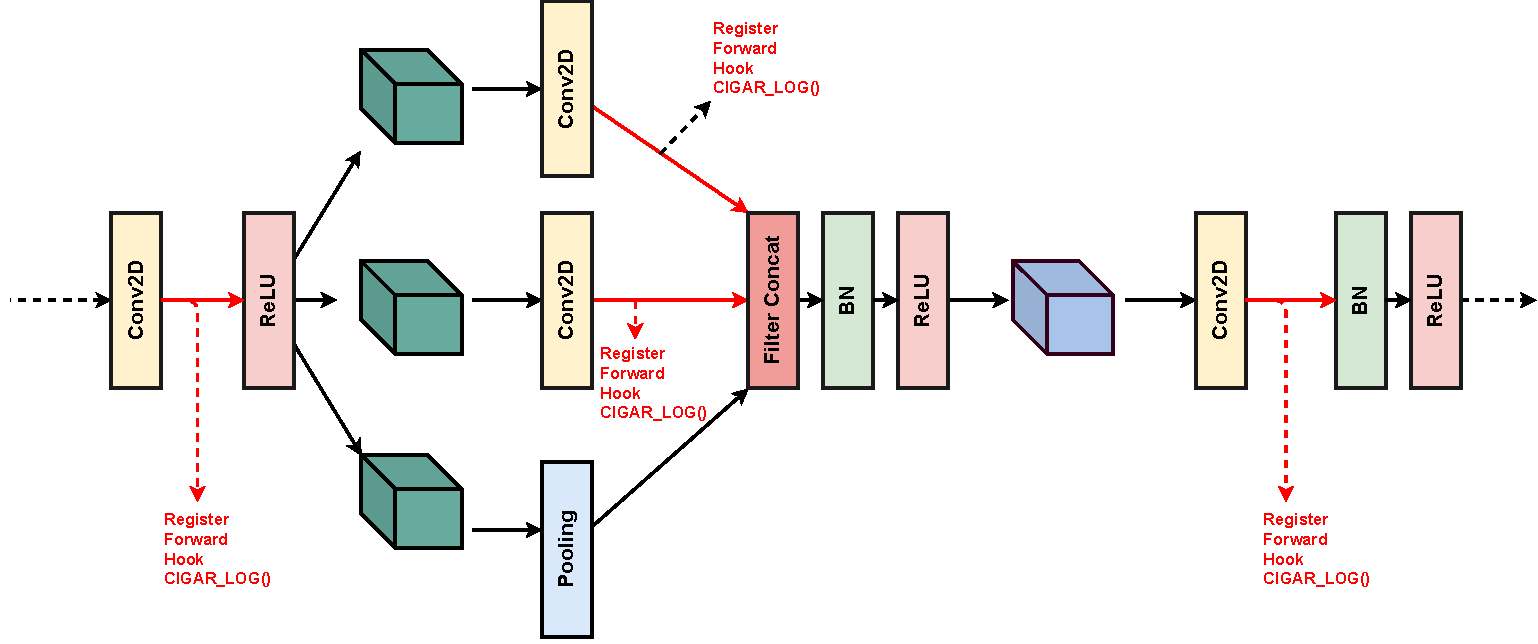
\includegraphics[scale=0.5]{fig/CIGAR.pdf}
    \caption{\ac{CIGAR} attachment of forward hooks to all model convolution layers}
    \label{fig:cigar_extraction}
\end{figure}

After all forward hooks are attached to the model, a forward pass of the model
is performed. Model layer statistics are added to the $model^{stats}_{dict}$ and
the collector's internal layer statistics tracker is reset. The layer statistics
collected for convolution layers are 1) the kernel sizes 2) strides 3) any additional padding
4) the number of convolution groups 5) kernel dilation. For linear layers the input and output feature sizes are collected.
For both layer types, input feature map dimensions are collected. 
After processing all of the models in $model_{dict}$, a $model^{stats}_{dict}$ is
returned for further analysis used to derive the necessary library insights for
pruning the dataflow design space. An illustration of that process is available
in \autoref{fig:cigar_flow}. New layers can be analysed by CIGAR provided that the
collector is updated to be able to collect statistics from different layer types
and Attach\_Collection\_Hooks is allowed to attach the collector's callback
function to the newly supported layer. 

\begin{figure}
    \centering
    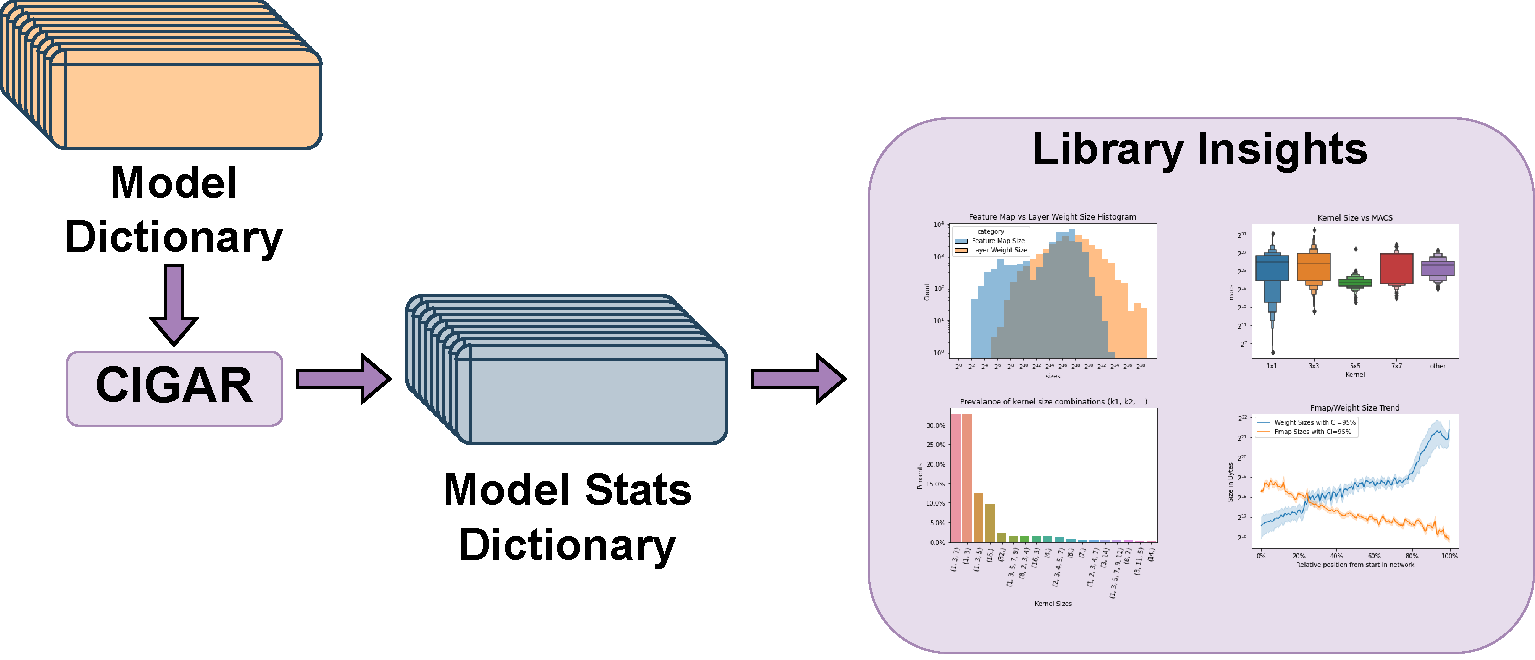
\includegraphics[scale=0.4]{fig/Cigar_flow.pdf}
    \caption{\ac{CIGAR} extraction of convolution layers}
    \label{fig:cigar_flow}
\end{figure}

\begin{algorithm}[H] 
    \caption{\ac{CIGAR}}
    \label{alg:cigar_algo}
    \begin{algorithmic}[1]
    \Require{$model_{dict}$} 
    \Ensure{$model^{stats}_{dict}$}
    \Statex
    \Function{Attach\_Collection\_Hooks}{$model, collector$}
        \State $hooks \gets []$
        \For{$layer \in model.named\_modules()$}
            \If{$type(layer)$ is $conv2d$ or $type(layer)$ is $linear$} 
                \State $hooks.push(layer.register\_forward\_hook(collector.layer\_collector))$
            \EndIf 
        \EndFor
    \State \Return{$hooks$}    
    \EndFunction
    \Statex
    \Function{Collect\_Library\_Statistics}{$model_{dict}$}
        \State $model^{stats}_{dict} \gets \{\}$
        \State $collector \gets Collector()$
        \For{$(model_{name}, model) \in model_{dict}$}
            \State $input\_img\_tensor \gets transform(open('default.jpg'), model)$
            \State $hooks \gets Attach\_Collection\_Hooks(model, collector)$
            \State $model.forward(input)$
            \State $model^{stats}_{dict}[model_{name}] \gets collector.model\_stats()$
            \State $collector.reset()$
            \State $hooks \gets Detach\_Collection\_Hooks(hooks)$
        \EndFor
        \State \Return {$model^{stats}_{dict}$}
    \EndFunction
    \end{algorithmic}
\end{algorithm}

\subsubsection{Neural Network Library Explored}
\label{chap:dda:dataflow_dse:pruning:cigar:library}

A diverse range of networks were explored by CIGAR for dataflow design space
pruning. The diversity of networks is reflected in the diversity of model types,
layer types, model sizes, and the number of MACs in the network. An illustration
of the model sizes vs number of MAC diversity is presented in
\autoref{fig:cigar_library_overview}. From \autoref{fig:cigar_library_overview}
it is clear that a wide range of models were selected as part of the CIGAR
library explored. The library includes smaller models like squeezenet and
mobilenetv2 as well as larger models like VGG16 \cite{dnn_is_sota_image}.
In terms of layer diversity the library includes conventional networks with both
convolution layers and linear layers as well as newer more exotic networks that
combine tranformer self attention layers with convolution layers like CoAtNet
\cite{xu_co-scale_2021}. An illustration of that layer type diversity is
reflected in figure \autoref{fig:cigar_library_overview}.b. A total of 695 networks where explored.
The full list of networks explored is available in the
appendix of this thesis. All models explored by CIGAR were implemented in
pytorch and provided by either torchhub in \cite{pytorch} or the PyTorch Image
Models (timm) package in \cite{timm}.  

\begin{figure}
    \centering
    \subfigure[]{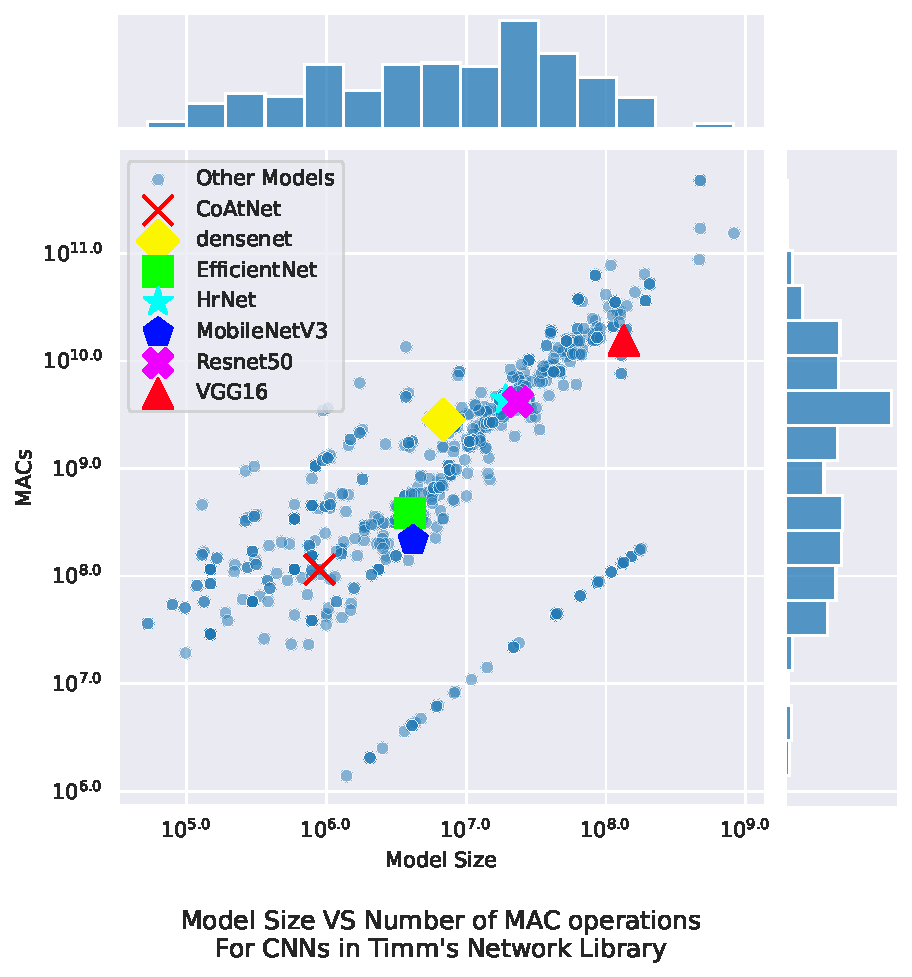
\includegraphics[width=0.495\textwidth]{Plots/overview/macs_vs_size.pdf}}
    \subfigure[]{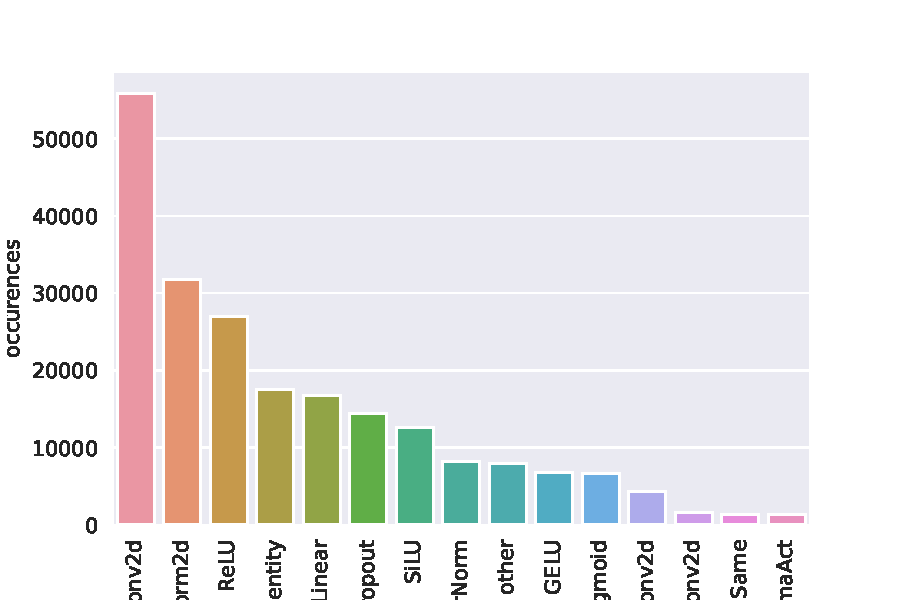
\includegraphics[width=0.495\textwidth]{Plots/overview/layer_types.pdf}}
    \caption{Illustration of CIGAR's library diversity based on (a) Model sizes and number of MACS (b) Model layer types}
    \label{fig:cigar_library_overview}
\end{figure}

\clearpage

\subsection{Applying CIGAR to prune the dataflow design space}
\label{chap:dda:dataflow_dse:pruning:applying_it}

\subsubsection{Loop Unroll Targets}
\label{chap:dda:dataflow_dse:pruning:applying_it:loop_unroll_targets}

The choice of loop unroll targets affects the stationarity of the data elements
in the convolution operation. For example, assuming a convolution layer with a
kernel size of (2, 2), if we unroll the F, C, KY, KX loops by a factor of 2,
weight element batches of size 16 will be loaded on to the chip in order to
compute the output feature map. These weight will remain stationary until all
input featuremap elements are loaded and consumed to evaluate the relevant
partial sums associated with the filter weights loaded. In this scenario, the
stationarity of the weight elements exceeds that of the input featuremap and
output featuremap elmements.   
We can determine determine what loop targets should be unrolled based on the
stationarity of each date type present in the convolution operation. A data
element that exhibits a high degree of stationarity should remain on chip for as
long as possible in order to minimize excessive reloads from off chip memory. We
can use the number of MAC operations a data element participates in as a
surrogate for stationarity. A data elements element reused accross many MAC operations
should be kept on chip for as long as possible to avoid excessive reloading of
that element from of-chip dram. Using CIGAR we can analyse data element reuse
behavior in all models of the TIMM library for the three data elements present in the convolution operation, input
feature maps elements (ifmaps), output feature map elements (ofmaps), and weight
elements. The results from this analysis are present in
\autoref{fig:reuse_behavior}. 

\begin{figure}
    \centering
    \subfigure[]{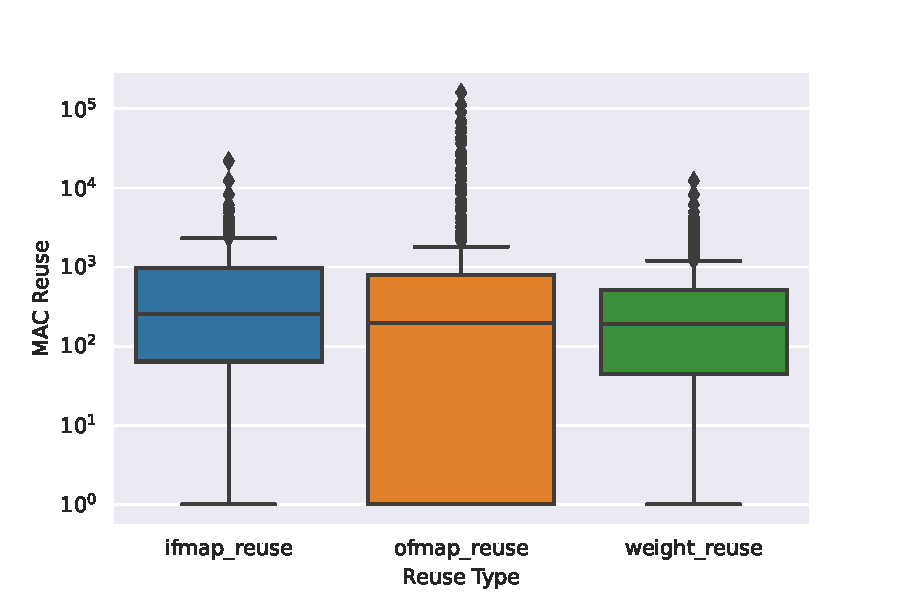
\includegraphics[width=0.495\textwidth]{Plots/reuse/reuse_box.pdf}}
    \subfigure[]{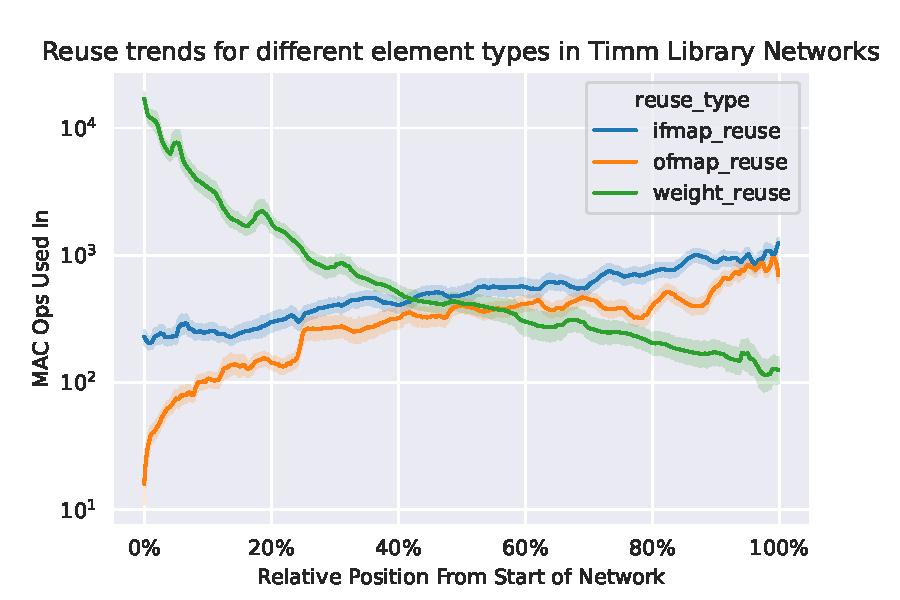
\includegraphics[width=0.495\textwidth]{Plots/reuse/reuse_trends.pdf}}
    \caption{Exploration of data element reuse behavior in convolution layers of models from the TIMM library, a) shows overall reuse behavior as a boxplot b) shows reuse behavior trends within models with multiple convolution layers}
    \label{fig:reuse_behavior}
\end{figure}


From \autoref{fig:reuse_behavior}.a the reuse
behavior between all three data elements is comparable with the exception ofmap
reuse having a much lower 0.25 quantile. Ifmap elements have a slightly higher
reuse with the median MAC operations performed per element load equal to 256
MACs. Weight and ofmap elements exhibit lower reuse at 192 and 196 MACs per
load. Reuse trends within networks show a general shift from high weight reuse
to high ifmap and ofmap reuse depending on the relative position from start
within a network. Weight reuse is initially almost 2 orders of magnitude higher
than ifmap and ofmap reuse, however, since the shift in reuse behavior happens
relatively early in most networks, higher ifmap reuse exceeding weight and ofmap
reuse persists for more layers within an network. These findings indicate that
all elements can exhibit a high degree of stationarity depending on the network and
even the layer position within a network. For an accelerator with a fixed
dataflow the choice of dataflow and hence which loops to unroll is heavily
influenced by the target networks expected to run on the accelerator.
The most flexible dataflow in this case is a weight stationary dataflow in which
the F, C, KY and KX loops are the unroll targets. This is due to the overlap
between weight stationary under 1x1 convolutions and GEMM discussed in (REF CHAP HERE), the choice of a weight
stationary dataflow lends itself well to \ac{GEMM} given the similarities in the
loop structure with regards to F and C loops for both applications. Furthermore,
a weight stationary based dataflow allows support for linear layers throught
this overlap which are quite prevelant in many moder networks as seen in
\autoref{fig:cigar_library_overview}.b. Given the flexibility of weight
stationary, F, C, KY and KX loops will be the loop unroll targets. This choice
of dataflow effectively creates two operational modes. A direct mode where
convolution operations with kernels that are supported directly are executed on
the accelerator and an indirect mode where kernels that are not supported directly are supported by
lowering/ lifting followed by conversion of the proceeding GEMM operation into a
1x1 convolution. A full explanation of indirect mode is given in
\autoref{chap:net_compile}. Note that convolution layers with non 1x1 strides are executed
under indirect mode. Supporting convolution layers with non 1x1 strides directly
is left as part of future work. From \autoref{fig:kernel_stats:strides} 1x1
strides are represent ~95\% of convolution layers so the implications of
indirect support of non 1x1 strides will likely be negligible when asscessing
the overall performance and energy efficiency of an accelerator implementing the
afformentioned operation modes.

% \clearpage
\begin{figure}
    \centering
    \subfigure[]{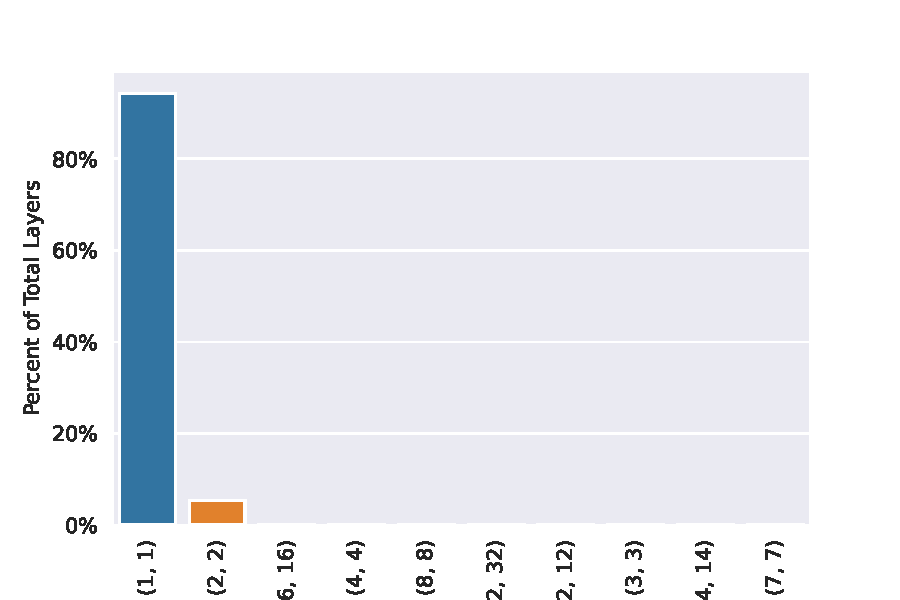
\includegraphics[width=0.495\textwidth]{Plots/kernel/strides.pdf}}
    \caption{Percentage of total layers in the TIMM library's networks that have a stride size (k, k)}
    \label{fig:kernel_stats:strides}
\end{figure}

% \clearpage
% \begin{lstlisting}[language=C, caption=Weight stationary dataflow, label={lst:conv_loop}]
% #pragma UNROLL F_UNROLL
% for(int f = 0; f < F; f+=F_UNROLL) // Filter loop
% #pragma UNROLL C_UNROLL
%     for(int c = 0; c < C; c+=C_UNROLL) // Channel loop
%         for(int y = 0; y < Y; y+=1) // Output feature map row
%             for(int x = 0; x < X; x+=1)  // Output feature map col
% #pragma UNROLL KY_UNROLL
%                 for(int ky = 0; ky < KY; ky+=KY_UNROLL)  // Kernel row
% #pragma UNROLL KX_UNROLL
%                     for(int kx = 0; kx < KX; kx+=KX_UNROLL)  // Kernel col
%                         O[f][y][x] += I[c][y+ky][x+kx]*W[f][c][ky][kx];
% \end{lstlisting}

% \begin{lstlisting}[language=C, caption=GEMM loops, label={lst:W_S_Generic_Loop}]
%     #pragma unroll F_UNROLL
%     for(int f = 0; f < F; f+=F_UNROLL) // Filter loop
%     #pragma unroll C_UNROLL
%         for(int c = 0; c < C; c+=C_UNROLL) // Channel loop
%             for(int z = 0; z < Z; z+=1)
%                 O[f][z] += W[f][z]*I[c][z];
% \end{lstlisting}

\subsubsection{Loop Unroll Factors}
\label{chap:dda:dataflow_dse:pruning:applying_it:loop_unroll_factors}

There exists significant variation with regards to the kernel sizes present in
the TIMM library. This makes the question of unroll factors and axis mapping for
the KY and KX loops more difficult.

From \autoref{fig:kernel_stats:freq}.a 1x1 and 3x3 kernel sizes dominate in
comparison to all other kernel sizes. This renders the choice of keeping KY and
KX loops folded impractical because if support is extended to an arbitrary K x K
kernel while KY and KX loops are folded the onboard storage for weights would
then need to be at least $K^2$ where $K$ is the upperbound of kernels supported
directly to avoid excessive weight fetches from DRAM. Unfortunatly, for ~80\% of
the layers in the network, that additional storage area would be significantly
underutilized by a factor of $\frac{1}{K^2}$ due to the overrepresentation of
1x1 kernels. To mitigate this underutilization of onboard memory for weights, KY
and KX loops need to be unrolled fully. However, this begs the question, what
kernel sizes should be assumed when unrolling the KY and KX loops? Any kernel
sizes assumed when unrolling KY and KX loops become kernel sizes that are
supported directly. Kernel sizes that are not assumed when unrolling KY and KX
loops can be supported indirectly through a lowering/lifting approach similair
to the ones discussed in \autoref{chap:background:intro}. This means that 1x1 kernels are assumed when
unrolling KY and KX loops, hence they have to be supported directly.
Other kernel sizes to support directly can be derived from
\autoref{fig:kernel_stats:freq}. In \autoref{fig:kernel_stats:freq}.b many networks contain at least 1 convolution
layer that is not 1x1 or 3x3. For example a 7x7 kernel exists in around ~20\% of
networks. The reason for the prevalance of 7x7 convolutions originates from the
historical use of resnet \cite{resnet} as a feature extractor for a significant
portion of networks analyzed by CIGAR.

\clearpage
\begin{figure}
    \centering
    \subfigure[]{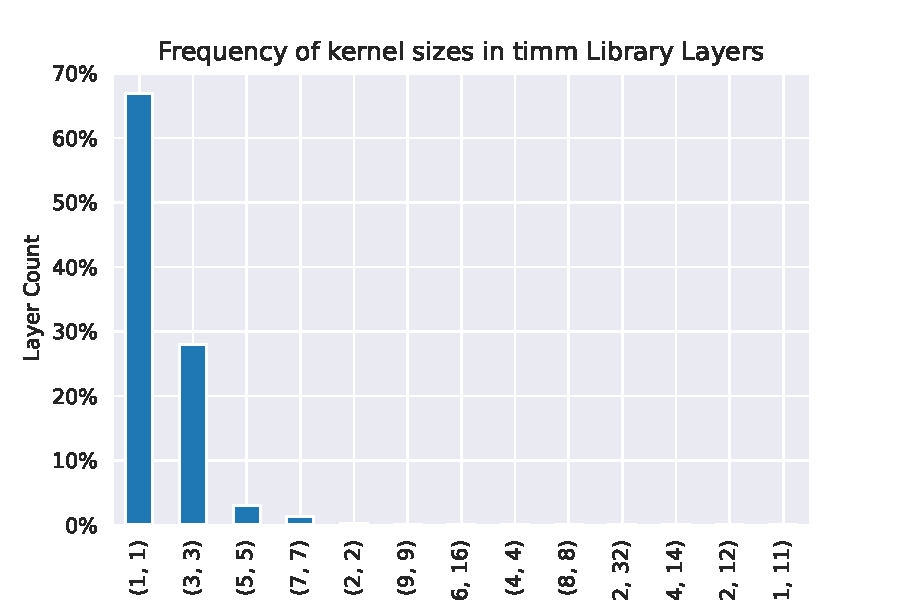
\includegraphics[width=0.495\textwidth]{Plots/kernel/freq.pdf}}
    \subfigure[]{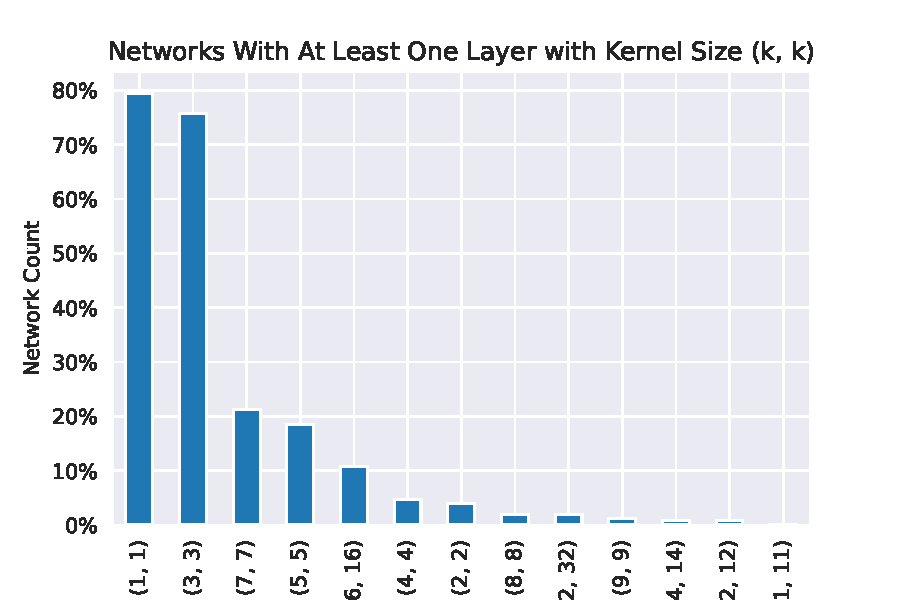
\includegraphics[width=0.495\textwidth]{Plots/kernel/at_least.pdf}}
    \caption{(a) Percentage of total layers in the TIMM library's networks that have a kernel size (k, k) (b) The percentage of networks in TIMM that have at least one kernel of size (k, k)}
    \label{fig:kernel_stats:freq}
\end{figure}


In \autoref{fig:kernel_vs_mac}.a, when adjusting for the the number of MACs
present in layers where these kernel sizes exist, 1x1 and 3x3 kernels share a
similar computational burden on the network with 1x1 having a much wider spread.
7x7 kernels have a much tighter spread but they still represent a similar
computational burden to 1x1 and 3x3 kernels in networks where they are present.
Adjusting for kernel frequency in \autoref{fig:kernel_vs_mac}.b, 1x1 and 3x3
kernels dominate all other kernel sizes in terms of number of MACs in most
network layers. From \autoref{fig:kernel_vs_mac} it is clear that 1x1 and 3x3
kernels need to be supported directly while all other kernels need to be
supported indirectly through a lifting/lowering approach like those discussed in
\autoref{chap:background:intro}. This limits the space of possible unroll
factors for the loop unroll targets and thus prunes the dataflow design space.
Supporting kernels indirectly will lead to an expansion of the IFmap due to the
duplication introduced by lowering, however that expansions is negligble given
the scarcity of non 1x1 and 3x3 layers. 

\clearpage
\begin{figure}
    % Todo: update figure titles to reflect origins of statistics
    \centering
    \subfigure[]{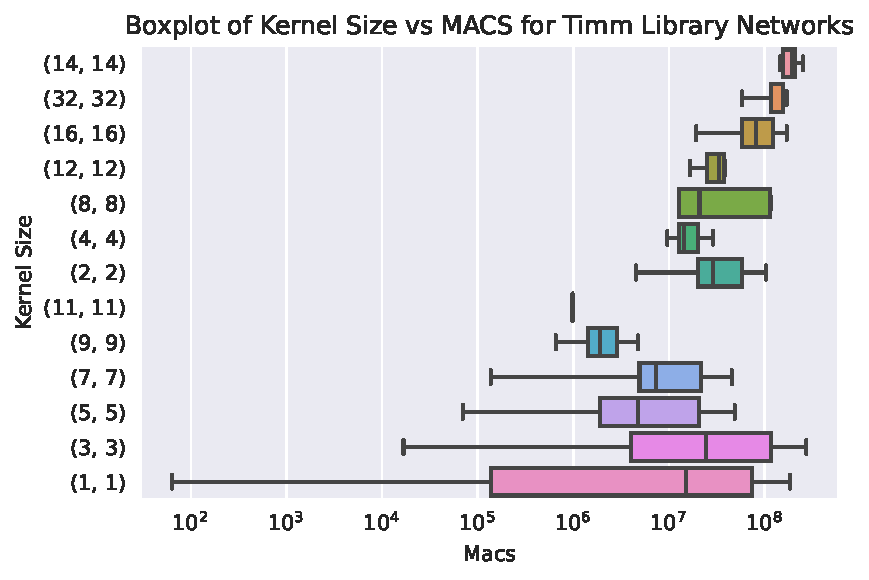
\includegraphics[width=0.495\textwidth]{Plots/kernel/macs.pdf}}
    \subfigure[]{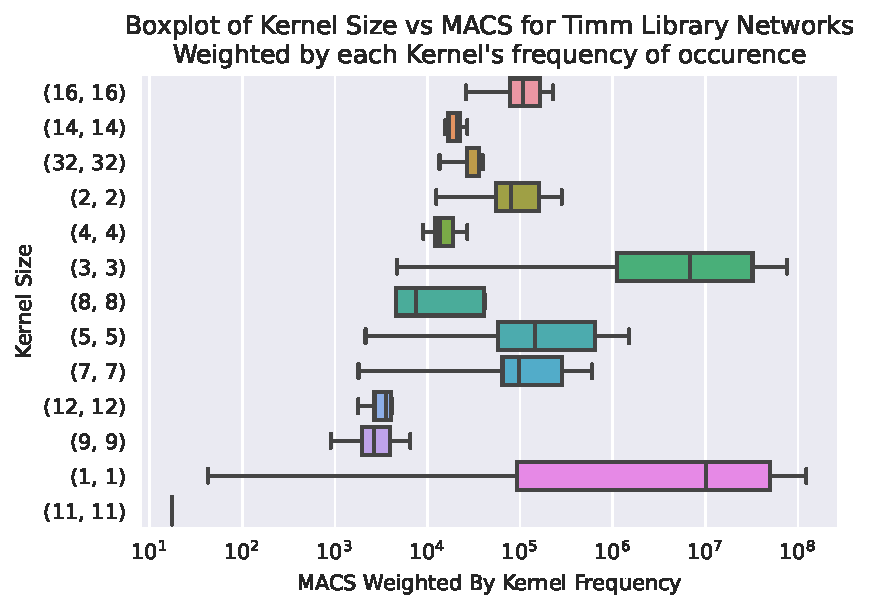
\includegraphics[width=0.495\textwidth]{Plots/kernel/macs_adjusted.pdf}}
    \caption{(a) Kernel size vs number of layer MACs  (b) Kernel size vs number of layer MACs adjusted by kernel frequency}
    \label{fig:kernel_vs_mac}
\end{figure}

% TODO: Introduce tiling discussion here using tiling figure
Depending on the chosen unroll factors, the architecture implementing the unroll
factors in effect tiles the weight tensor and processes it tile by tile in the
convolution operation. An
illustration of this concept is present in
\autoref{fig:tiling_connection_to_unroll_targets}. Loop unroll factors determine
PE allocation 
Tiling of a weight tensor arises from the processing of filters, channels and
kernels in batches whose size depend on the unroll factors. 
Padding of a weight tensors is performed wherever the chosen PE
binding for filter or channel loops exceeds the number of channels and filters
being processed in the tile. In
\autoref{fig:tiling_connection_to_unroll_targets} a weight tensors of dimension
$R^{6\times 3\times 2\times 2}$ is tiled with $F_{unroll} = 4$, $C_{unroll}=8$,
$K_{unroll}=2$ with kernel loops mapped to the horizontal axis alongside channel
loops. Additional padding in the horizontal and verticle axis is added given
excess allocation of PEs in both spatial axis in all tiles except the top left
one. This representation of the weight tensor as a series of tiles processed by
the architecture is useful when considering the scheduling of a convolution
operation in a network. Tiling of weights and their effect on scheduling is
discussed in \autoref{chap:net_compile}.

\begin{figure}[]
    \centering
    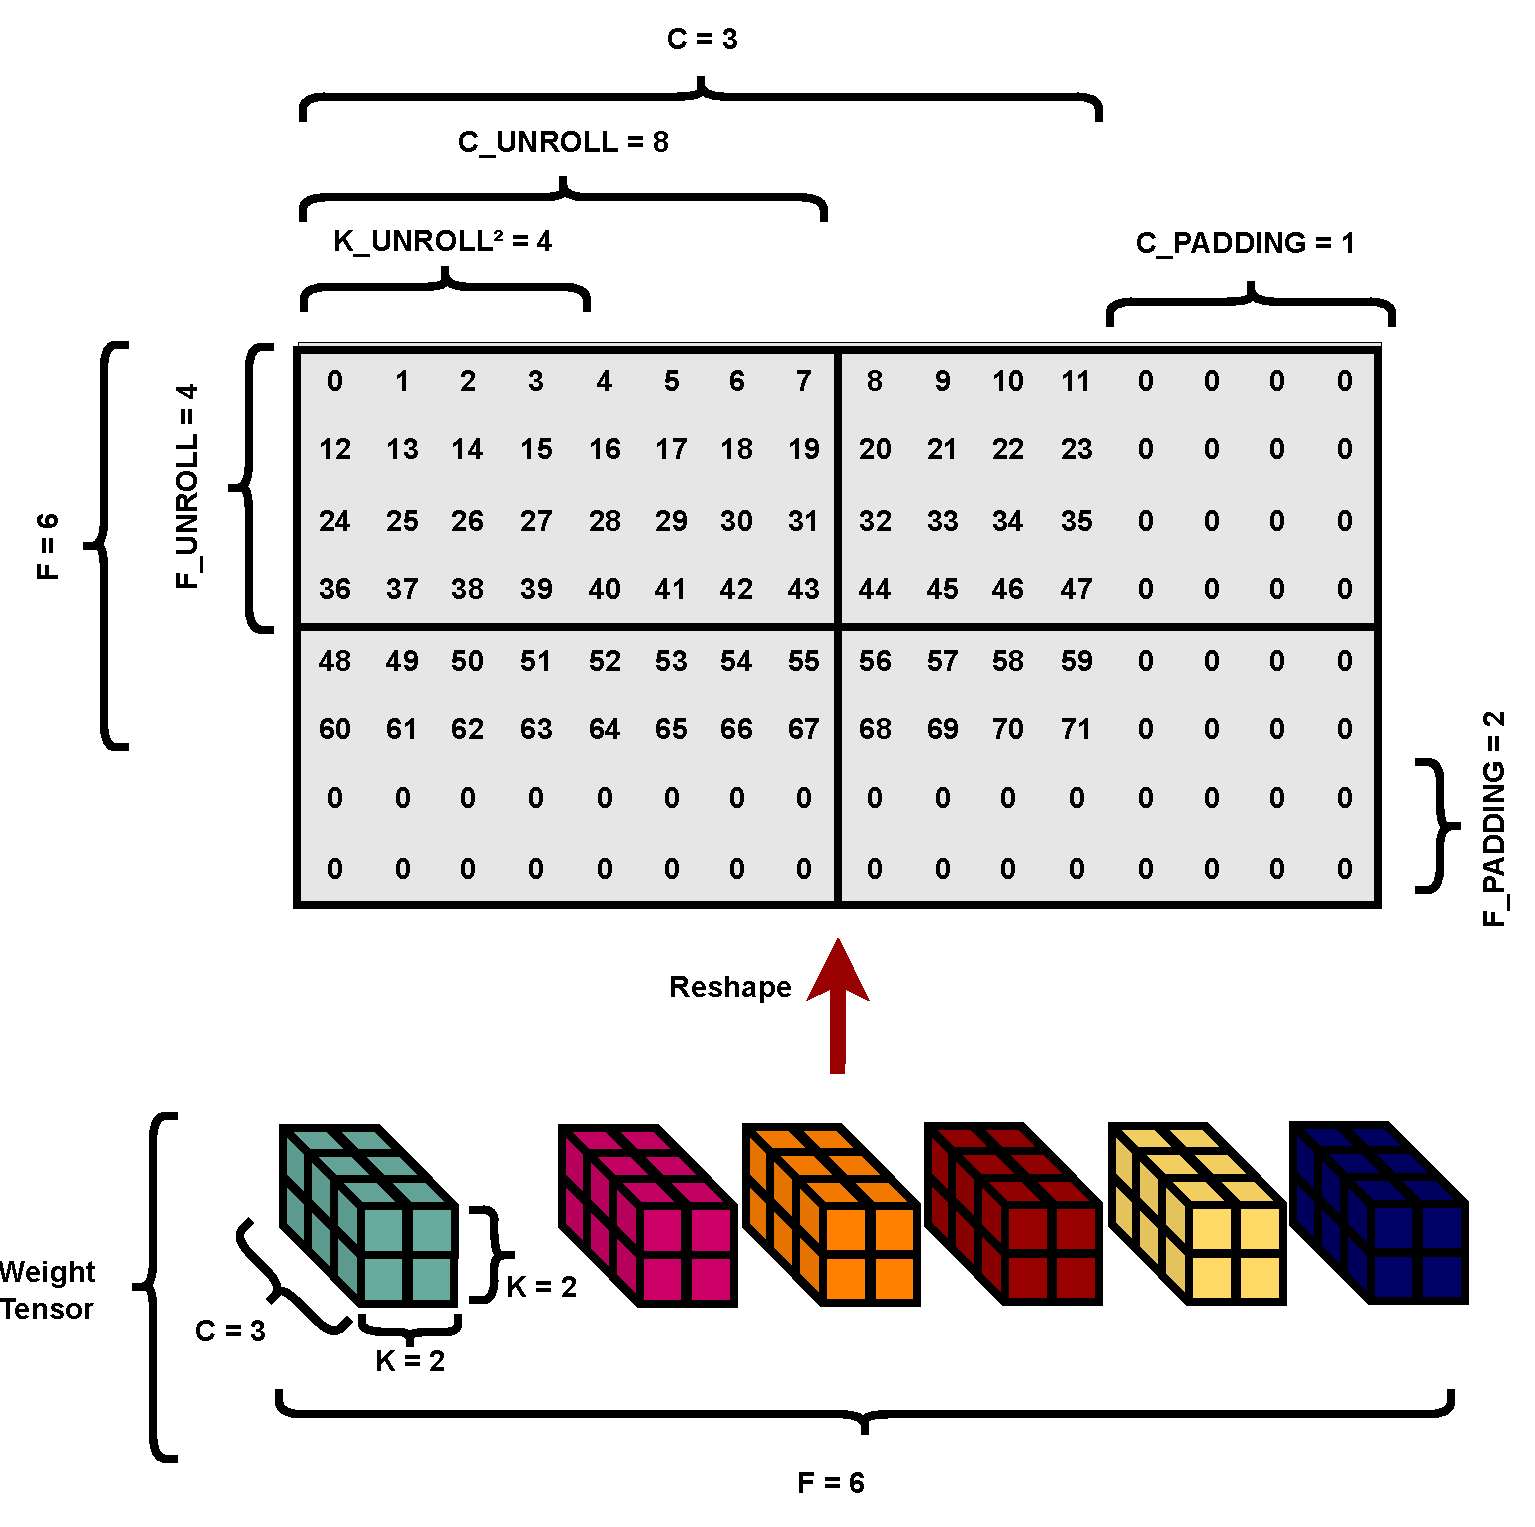
\includegraphics[scale=0.5]{fig/tiling.pdf}
    \caption{An illustration of weight tiling by loop unroll factors}
    \label{fig:tiling_connection_to_unroll_targets}
\end{figure}

\clearpage 

% \subsubsection{Loop ReOrdering}
% \label{chap:dataflow_dse:pruning:applying_it:loop_ordering}

% % In the final template there are 4 template parameters that are customizable
% % depending on the target performance/area/energy efficiency requirements of the
% % acclerator. The first and the second are the unroll factors for filters
% % ($F_{unroll}$) and channels ($C_{unroll}$). The third is the set of directly
% % supported kernels. Finally the fourth is the spatial axis mapping of the kernel
% % loops ($K_{axis}$). Each of these parameters has an effect on on-chip storage
% % required for the different memories accessed.

% \begin{figure}
%     \centering
%     \subfigure[]{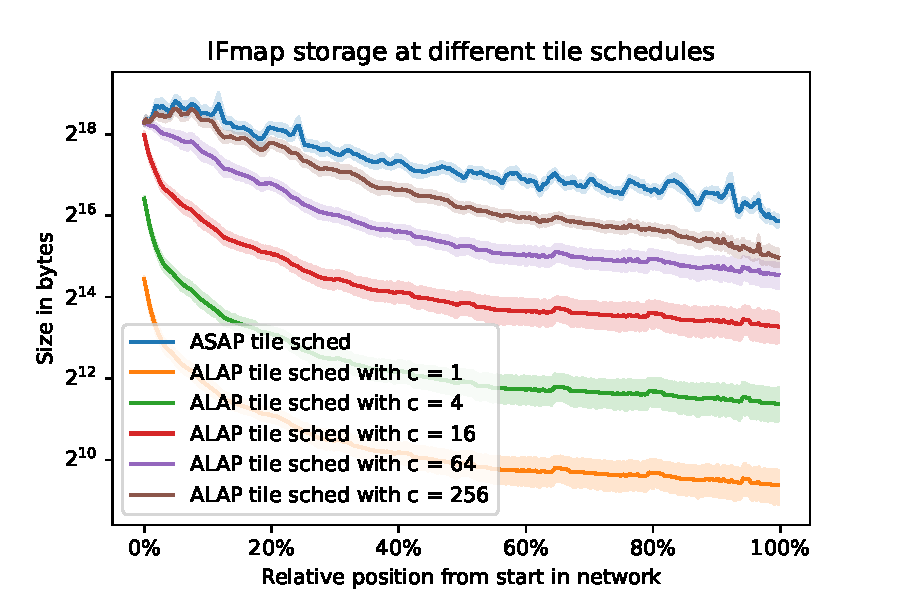
\includegraphics[width=0.45\textwidth]{Plots/ifmap_Storage.pdf}}
%     \hspace{0.1cm} 
%     \subfigure[]{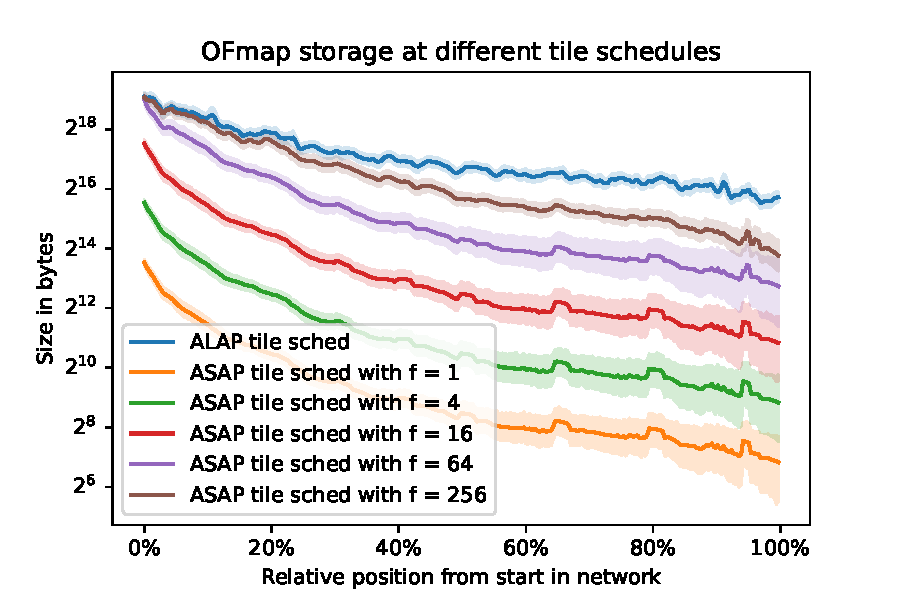
\includegraphics[width=0.45\textwidth]{Plots/PSUM_Storage.pdf}}
%     \subfigure[]{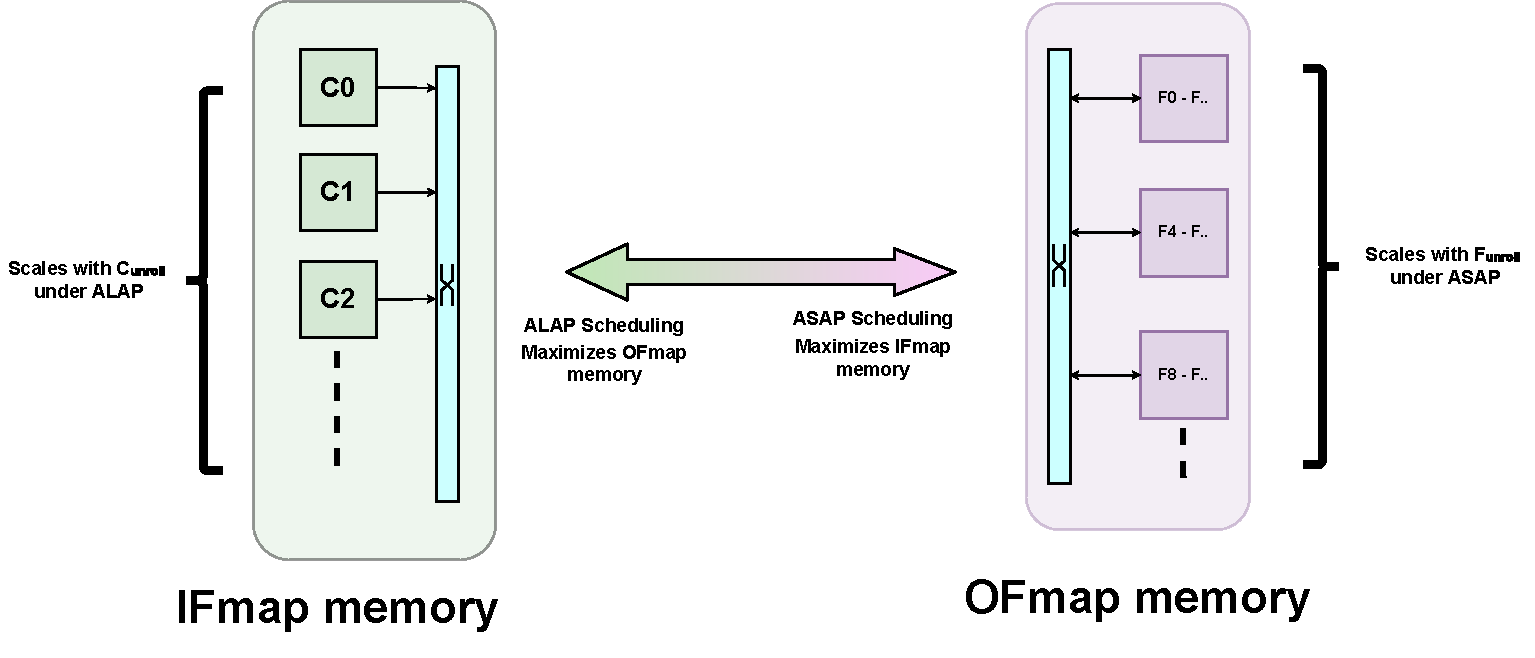
\includegraphics[width=1\textwidth]{fig/psum_ifmap_mem_scaling.pdf}}
%     \caption{Illustration of storage tradeoff between OFmaps and IFmaps depending on tile scheduling (loop ordering) and accelerator template parameters (loop unroll factors) (a) IFmap storage (b) OFmap storage (c) archictural illustration}
%     \label{fig:Fmap_scaling}
% \end{figure}

% \begin{figure}
%     \centering
%     \subfigure[]{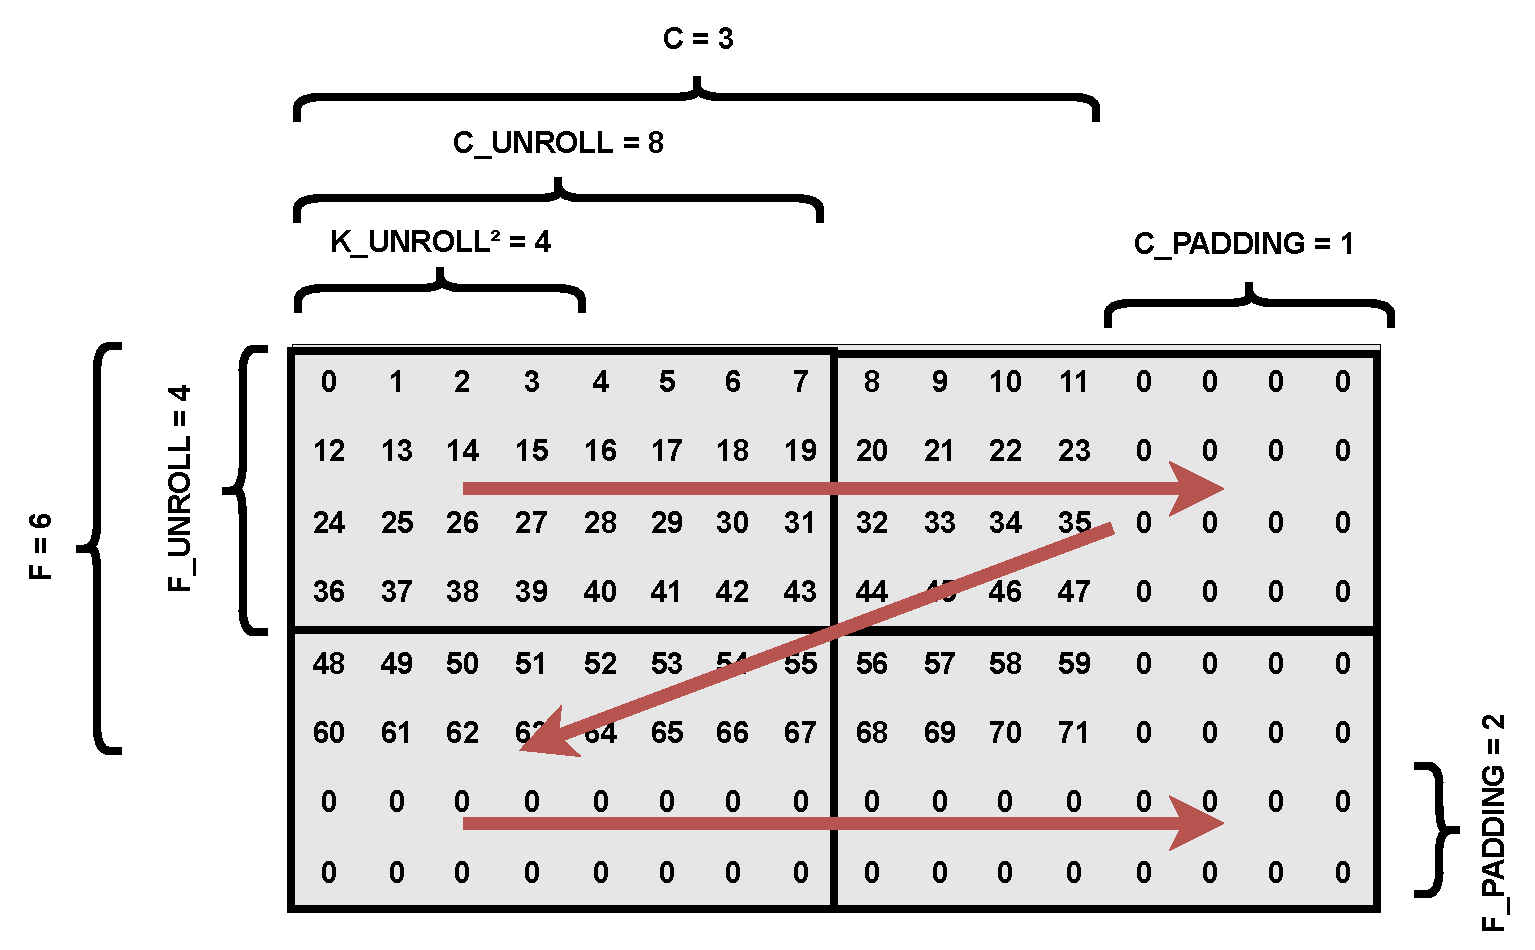
\includegraphics[width=1\textwidth]{fig/asap_tiling.pdf}}
%     \hspace{0.1cm} 
%     \subfigure[]{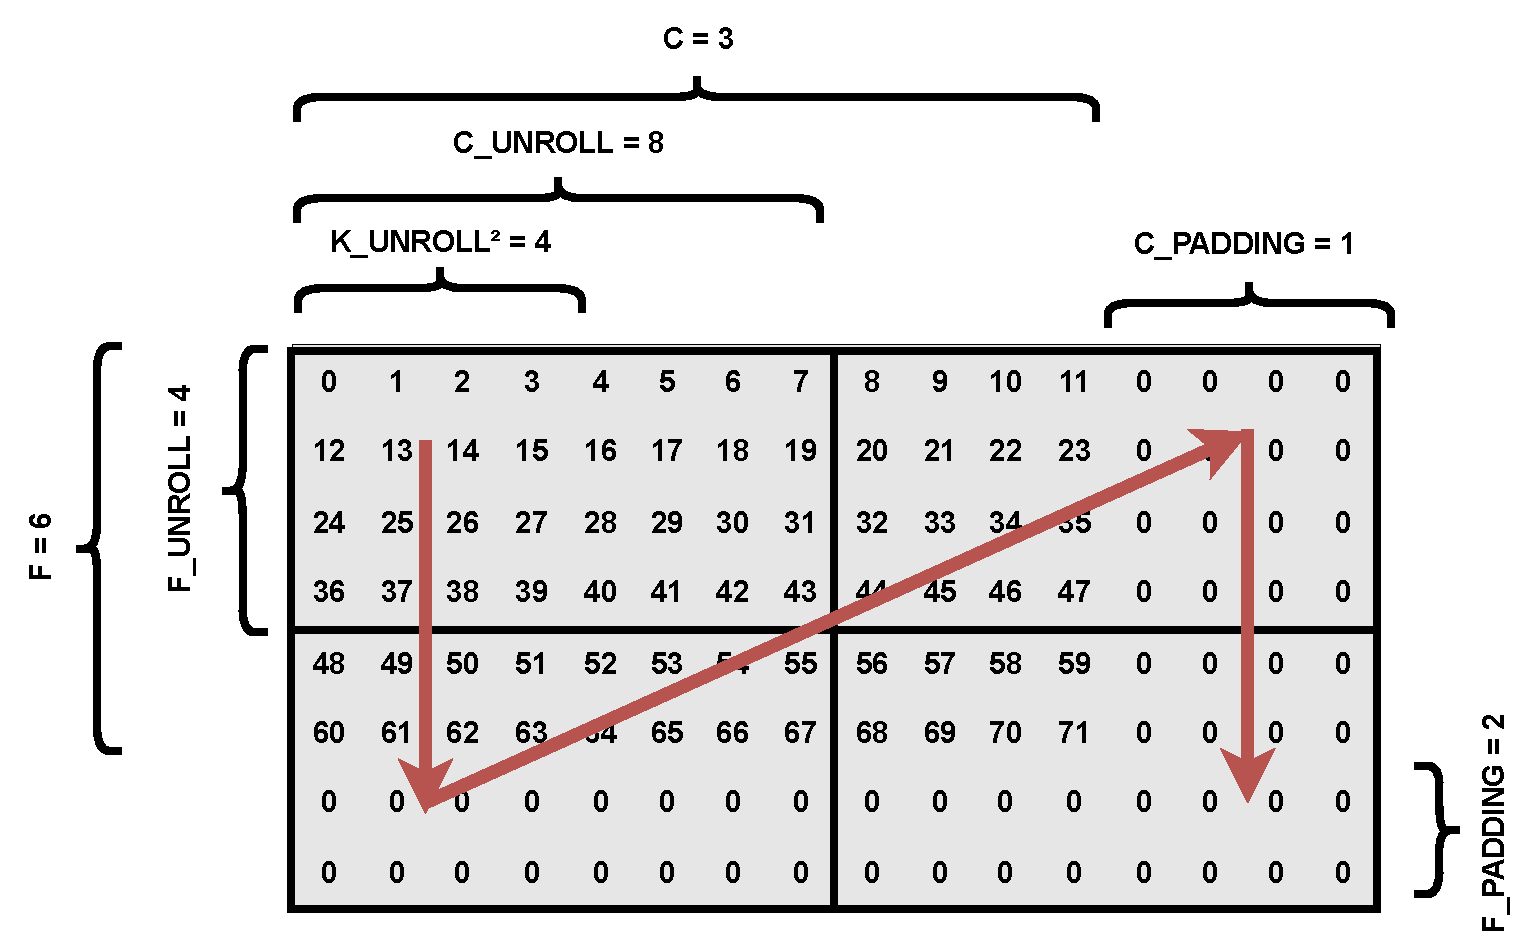
\includegraphics[width=1\textwidth]{fig/alap_tiling.pdf}}
%     \caption{Illustration of different tiling schedules (a) ASAP scheduling (F, C)  (b) ALAP scheduling (C, F)}
%     \label{fig:tile_scheduling}
% \end{figure}


% While a weight stationary offers limited flexibility with regards to loop
% reoredering it does offer some degree of flexibiltiy with regards to ordering
% filter loops and channel loops. F, C loop ordering affects required on-chip
% storage for IFmaps and OFmaps.
% Under Direct mode and Gemm mode with balanced lowering, IFmap sizes
% do not exceed $2^{19.25}$ bytes (assuming 8 bit precision) for 95\% of all
% convolution layers in CIGAR's library. An estimation of the
% on-chip area required to store IFmaps using the model presented in
% \cite{area_model} yields a total on-chip area per sram bit stored equal to 0.013
% $um^2$ which translates to $0.064 mm^2$ on-chip area dedicated to sram buffers
% for storing entire input feature maps for a layer at 14nm technology.
% This area/storage does not scale with increased/decreased filter unroll factor,
% channel unroll factor or max directly supported kernel size. On-Chip area
% dedicated to storing Weights scales with the afformentioned parameters.
% Storage with regards to OFmaps depends on the loop ordering in the chosen
% dataflow. Specifically on-chip OFmap storage depends on whether filter loops and
% channel loops are reordered such that OFmaps are retired as fast as possible
% (ASAP tile scheduling) by iterating through IFmap channels first while
% processing a groups of filter, or as late as possible (ALAP tile scheduling) by
% iterating through filters first while processing a group channels. These two
% orderings for filter loops and channel loops represent different tile schedules
% for processing convolution layers. An illustration of both tile scheduling
% approaches is illustrated in \autoref{fig:tile_scheduling}. In
% \autoref{fig:tile_scheduling} a 1x1 convolution layer's weights are shown with
% the architecture's unroll factors overlayed on top. The overlay of the
% architecture's unroll factor creates distinct weight tiles where componenets of
% the OFmap are computed. The order of executing these weight tiles depends on the
% chosen tile schedule. ASAP which represents F, C loop ordering and ALAP which
% represents C, F loop ordering. 

% A tradeoff between required IFmap storage and required OFmap storage is apparent
% in \autoref{fig:fmap_size_trends}. Under ASAP scheduling, storage requirements for
% OFmaps scales with $F_{unroll}$ because $F_{unroll}$ represents the maxmimum
% number of filters in flight. Storage requirements for IFmaps is maximized under
% ASAP because all channel data would need to be held on-chip assuming no
% additional reads can be made from DRAM for IFmap channels. Under ALAP
% scheduling, storage requirements for IFmap scale with $C_unroll$ because
% $C_{unroll}$ represents the maximum number of channels in flight. Storage for
% OFmaps is maximized under ALAP. In this thesis it is assumed that chip
% area (and thus on-chip memory) is always sufficient at least one of the
% afformentioned tile schedules without requiring loop blocking and additional
% DRAM accesses for feature maps. An exploration of the effect of loop blocking
% under more restrictive area constraints is relegated to future work. 

% \clearpage

\section{Exploring The Hardware Implementation Design Space}
\label{chap:dda:hw_dse}

Based on the conclusions derived from \autoref{chap:dda:dataflow_dse:pruning},
weight stationary is the most flexible dataflow choice given the overlap between
under 1x1 convolutions and GEMM. This gives rise to an accelerator with two
operational modes, direct Mode where a subset of possible kernel sizes are
supported and GEMM mode where all other kernel sizes and strides are supported
in via lowering/ lifting based approach. In this section we will determine an
appropriate hardware implementation for the weight stationary dataflow chosen in
\autoref{chap:dda:dataflow_dse:pruning:applying_it} using the hardware
implementation taxonomy from \cite{maestro}, Based on the reuse and
communication behavior of the different elements (ifmap, ofmap and weights) in a
convolution operation using weight stationary we can infer the appropriate
hardware implementation for on-chip communication and memory from
\cite{maestro}. To perform this deduction we will use the polyhedral model to
analyse temporal reuse in \autoref{chap:dda:hw_dse:temporal_analysis} and
spatial reuse in \autoref{chap:dda:hw_dse:spatial_reuse_analysis}. Based on the
analysed reuse behavior an initial hardware implementation for HERO will be
given and further improved after applying a simplification of the on-chip memory
hierarchy in \autoref{chap:dda:hw_dse:simplifying_hierarchy}. The final hardware
implementation for HERO will be given in \autoref{chap:dda:hw_dse:final}.

\subsection{Temporal Reuse Analysis}
\label{chap:dda:hw_dse:temporal_analysis}

Unrolling convolution dataflow loops yield multiple instances of the \ac{MAC}
statement present in the original convolution nested loops in
\autoref{lst:conv_loop}. These statements represent \ac{PE}s performing MAC
operations concurrently. 
\ac{MAC} statement instances can be distinguished from eachother based on the memory access offsets that
exist in them as a result of unrolling filter, channel and kernel loops. For
unroll factors F\_T for filters, C\_T for channels, KY\_T and KX\_T for kernels
each statement will have a coresponding access offset based on the statement
index $j \in [0, F\_T*C\_T*KY\_T*KX\_T]$ for each of the data elements
(IFmap, OFmap and Weights) accessed in the loop body. Each \ac{MAC} statement
at index j is characterized by a set of access offsets {Fj, Cj, KYj,
KXj} used by the memory accesses in the \ac{MAC} statement. Applying the unroll
factors and distinguishing each \ac{MAC} statement based on it's statement index
j yields the loop configuration in \autoref{lst:conv_loops_unrolled}. 

\begin{lstlisting}[language=C, caption=Fully unrolled convolution dataflow loops, label={lst:conv_loops_unrolled}]
    for(int f = 0; f < F; f+=F_T) // Filter loop
        for(int c = 0; c < C; c+=C_T) // Channel loop
            for (int y = 0; y < Y; y++) // FeatureMap Height
                for(int x = 0; x < X; x++) // FeatureMap Width
                        ...
                        /* For all j in [0, F_T*C_T*KY_T*KX_T[ */ 
                        O[f+Fj][y][x] += W[f+Fj][c+Cj][KYj][KXj]* \
                                            I[c][y+KYj][x+KXj] 
                        ...
\end{lstlisting}

Each MAC statement is composed of three seperate memory accesses for ifmap,
ofmaps and weights. For each of those memory access has a temporal index (it's location in time) defined by the
iteration domain vector $[f, c, y, x, ky, kx]$. A mapping exists between each
iteration domain vector and MAC statement's memory accesses.  
Temporal reuse analysis for each of the memory accesses in the MAC statements is performed on the loops in \autoref{lst:conv_loops_unrolled}. The different
operational modes (Indirect/ Direct) are analysed concurrently using the same loop
representation as they only differ based on whether we set the width loop
upperbound to 1, and set the kernel loops upper bounds to 1. Since
kernel loops are always unrolled fully this sets KY\_T and KX\_T to 1. We can
analyse temporal reuse in the dataflow represented in
\autoref{lst:conv_loops_unrolled} by adapting the approach in \cite{meeus} 
to the afformentioned dataflow iteration domain and access functions.
Given iteration domain restrictions imposed by the polyhedral model,
\autoref{lst:poly:analysis} assumes unroll factors F\_T =
C\_T = 4. Setting F\_T and C\_T to concrete values does not overall reuse behavior during temporal reuse analysis.

\clearpage
\begin{lstlisting}[caption=Polyhedral analysis of reuse in iscc for convolution loops, label={lst:poly:analysis}]
    // Define iteration domain for all accessed data elements
    ID:=[F, C, Y, X] -> { S[f, c, y, x] : 0<=f<F and 0<=c<C and f mod 4=0 and c mod 4=0, 0<=y<Y and 0<=x<X};
    // Define access functions for each data element
    IFMAP:=([Cj, KYj, KXj] -> {S[f, c, y, x] -> IF[c+Cj][y+KYj][x+KXj]})*ID;
    OFMAP:=([Fj] -> {S[f, c, y, x] -> PS[f+Fj][y][x]})*ID;
    WEIGHT:=([Fj, Cj, KYj, KXj] -> {S[f, c, y, x] -> W[f+Fj][c+Cj][KYj][KXj]})*ID;
    // Evaluate temporal reuse
    IFMAP_REUSE:=(IFMAP.(IFMAP^-1))*(ID<<ID);
    OFMAP_REUSE:=(OFMAP.(OFMAP^-1))*(ID<<ID);
    WEIGHT_REUSE:=(WEIGHT.(WEIGHT^-1))*(ID<<ID);  

\end{lstlisting}

In \autoref{lst:poly:analysis}, the iteration domain for the loops in
\autoref{lst:conv_loops_unrolled} is converted into it's set representation in
line 2 where for some access statement S the loop iteration vector [f, c, y, x,]
is bound by the upper and lower bounds [0, F], [0, C], [0, Y], [0, X]
respectively. These bounds are represented by the associated parameters passed
to the iteration domain set assignment in line 2. 

Each memory accessed for ifmaps, ofmaps and weights in each MAC statement has
an associated memory access function. 

Each instance of the loop iteration vector [f, c, y, x]
is mapped to a memory access for each of the memories in lines 4-6. Access
offsets used in the memory access functions are passed as parameters based on
the convention established in \autoref{lst:conv_loops_unrolled}. This mapping
creates multiple temporal instances for each memory access in each \ac{MAC}
statement instance.  For
example, for example, the OFmap access that occurs at iteration vector [f = 2, c= 1, y = 0,
x = 1] is a different temporal instance of the same OFmap access at [f = 1, c = 1,
y = 0, x = 1]. 
Two accesses that access the same index but at different
iteration vectors are different temporal instances of the same access.
After applying the operation in lines 8-10, we can determine the
temporal reuse behavior of the accessed memories in the convolution loops.  
\autoref{lst:poly:result} shows the reuse behavior for each memory. Original
iteration domains constraints are ommited for brevity. The operation in lines
8-10 map all iteration domains to all proceeding iteration domains that access
the same memory locations for each of the data elements.

\clearpage
\begin{lstlisting}[caption=Polyhedral analysis results w.r.t data elements in convolution loops, label={lst:poly:result}]
    IFMAP_REUSE;
    [F, C, Y, X, Cj, KYj, KXj]->{
        S[f, c, y, x] -> S[f', c' = c, y' = y, x' = x] :
            ... f' > f and 0 <= f' < F ... 
        }
    OFMAP_REUSE;
    [F, C, Y, X, Fj]->{ 
        S[f, c, y, x] -> S[f' = f, c', y' = y, x' = x] : 
            ... c' > c and 0 <= c' < C ... 
        }
    WEIGHT_REUSE;
    [F, C, Y, X, Fj, Cj, KYj, KXj] -> { 
        S[f, c, y, x] -> S[f' = f, c' = c, y', x'] : 
            ... y' > y and 0 <= y' < Y and 0 <= x' < X ...; 
    }
\end{lstlisting}

\autoref{lst:poly:result} shows the temporal reuse behavior in memory accesses. For each
of the memories accessed (IFmap, OFmap and Weights) there exists a set of reuse
(IFMAP\_REUSE, OFMAP\_REUSE and WEIGHT\_REUSE) maps that map each iteration
vector of an access to all the proceeding iteration vectors where that same
access occurs. From the above listing we can see that, in the set of IFmap reuse
maps (IFMAP\_REUSE), IFmap channels are reused temporally with respect to filter
loops. For a given IFmap accessed at channel c, that channel is accessed again
when computing the output for all proceeding filter loop iterationtions f' where
$f'>f$. The absence of other mappings in the set of reuse maps IFMAP\_REUSE shows
that 1) this reuse behavior holds at any arbitrary iteration vector [f, c, y, x]
and 2) this reuse behavior depends only on the filter loop. For the set OFmap
reuse maps (OFMAP\_REUSE), for an OFmap acceess at iteration vector [f, c, y,
x], it is accessed again at loop iteration f'=f, c', y'=y, x'=x where $c'>c$.  
For (WEIGHT\_REUSE) Weights exhibit temporal reuse w.r.t feature map width and
height, the X and Y loops. 

Applying the hardware taxonomy in \cite{maestro}, IFmap exhibits temporal reuse,
multicast communication given their repeated read only behavior. OFmap exhibits temporal reuse, reduction communication
given their read-modify-write behavior. Weights exhibit temporal multicast
communication. Given the limited implementation options derivable from temporal
reuse we can comfortably define the appropriate connectivity and memory
hierarchies for IFmaps channels, OFmaps channels (equivelent to number of
Filters), and Weights. The beginings of a hardware template derived from the
afformentioned temporal reuse behavior of the different memories referenced in
the convolution dataflow can be seen in \ref{fig:reuse_illus}. In
\ref{fig:reuse_illus} the template is broken into 3 major componenets. The first
is the IFmap memory hierarchy currently with only 1 level. The 2nd component is
the compute portion of the template where partial sums are computed and
aggregating into OFmap data elements. Finally the 3rd component which is the
OFmap memory that stores OFmap partial sums until they are aggregated into OFmap
pixels and are written back to memory.

\begin{figure}[]
    \centering
    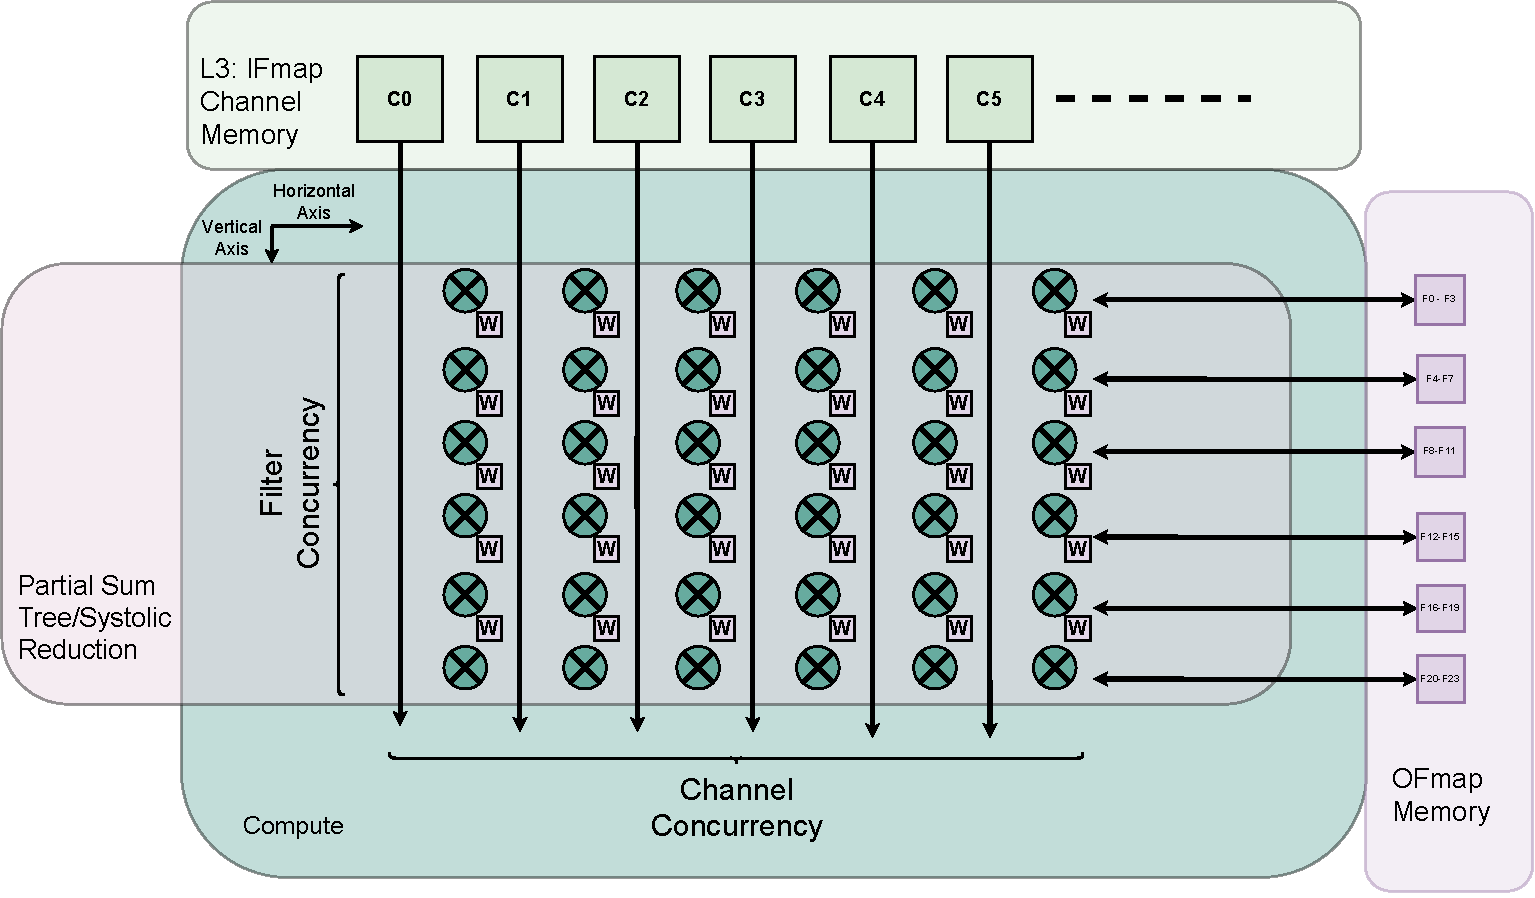
\includegraphics[scale=0.4]{fig/reuse_illus.pdf}
    \caption{Initial hardware template incorporating buffers IFmap and OFmap temporal reuse}
    \label{fig:reuse_illus}
\end{figure}

In addition to the temporal reuse behavior exhibited across IFmap channels,
temporal reuse exists within individual IFmap channels due to the stencil based
access pattern arising from the X, Y, KY, KX loops in the dataflow. That
temporal reuse is affected by the decision to fully unroll kernel loops which
causes temporal reuse to exist between unrolled different PEs processing the
same kernel. Proof of the existence of that temporal reuse is given in the polyhedral analysis in
\autoref{lst:poly:xy_reuse}. 

\begin{lstlisting}[caption=Analysis of IFmap channel reuse, label={lst:poly:xy_reuse}]
    ID_XY:=[Y, X, KY, KX] -> { S[y, x, ky, kx] : 0<=ky<KY and 0<=kx<KX and 0<=y<Y and 0<=x<X};
    IFMAP_XY:=({S[y, x, ky, kx] -> IF[y+ky][x+kx]})*ID;
    IFMAP_REUSE_XY:=(IFMAP_XY.(IFMAP_XY^-1))*(ID_XY<<ID_XY);
    IFMAP_XY_REUSE;
    [Y, X, KY, KX] -> { 
        S[y, x, ky, kx] -> S[y', x', ky' = (y - y') + ky, kx' = (x - x') + kx] : 
            ... y' > y and (y + ky) -KY < y' <= (y + ky) and (x + kx) -KX < x' <= (x + kx) ...;
    }
\end{lstlisting}

\begin{figure}[]
    \centering
    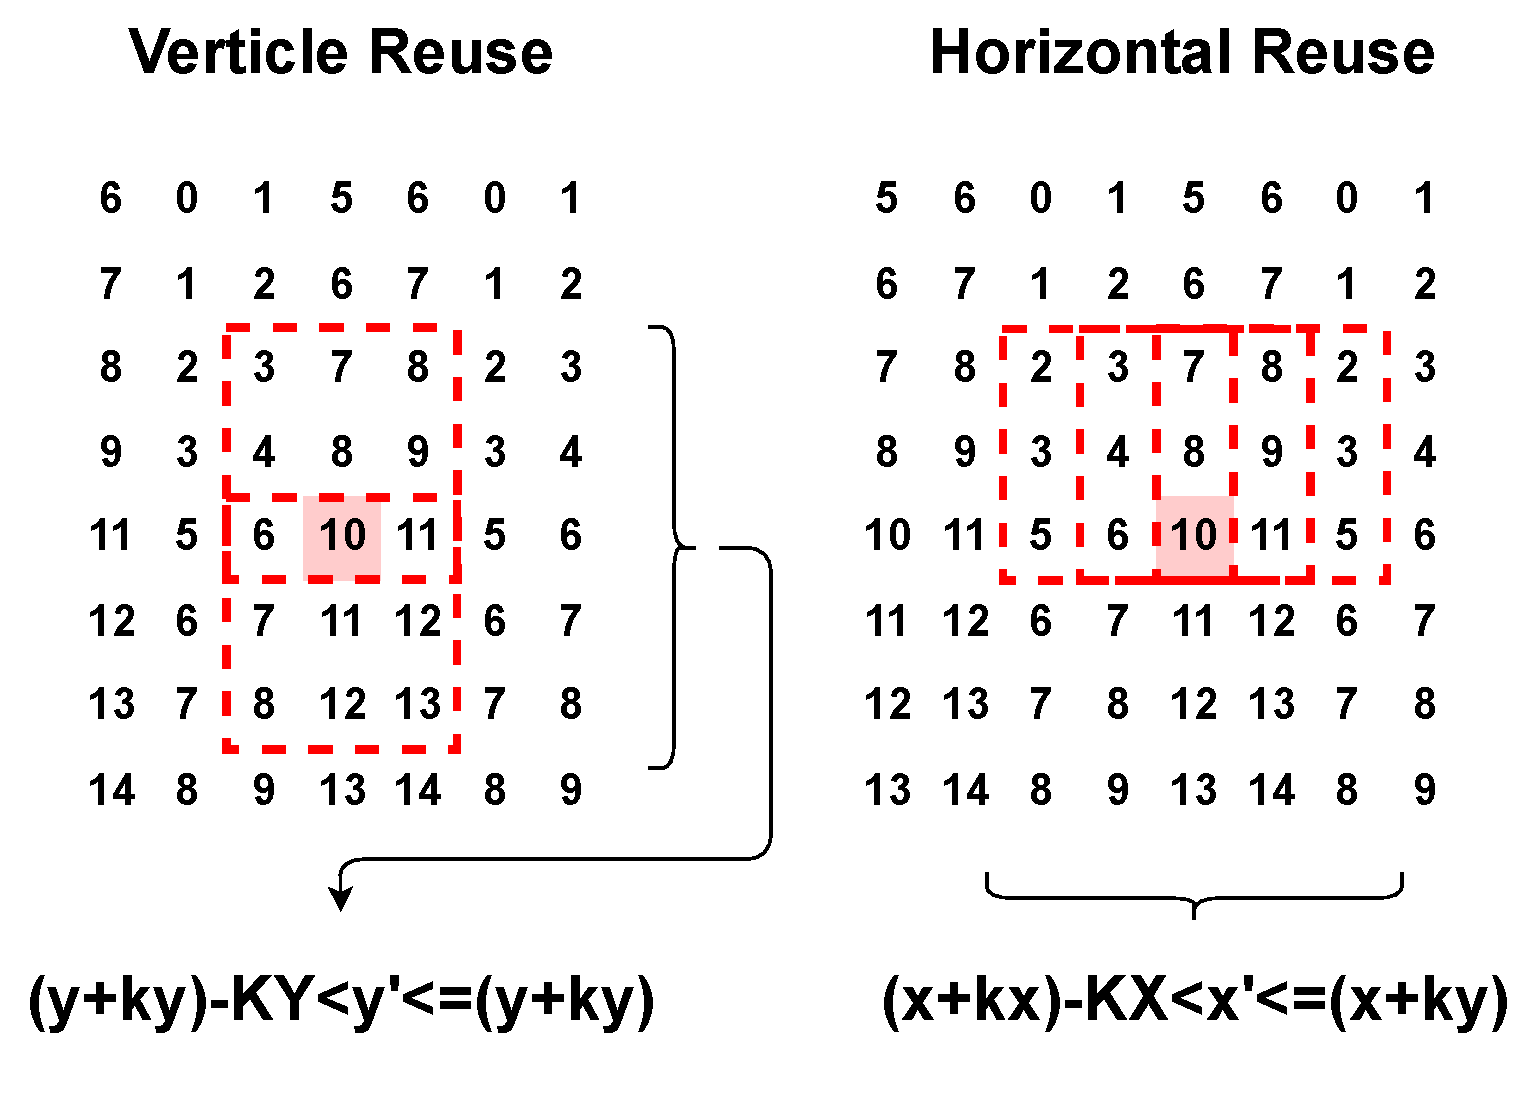
\includegraphics[scale=0.4]{fig/xy_reuse.pdf}
    \caption{IFmap Reuse Behavior w.r.t individual feature map channels}
    \label{fig:ifmap_xy_reuse}
\end{figure}

Within an individual IFmap channel, temporal reuse is exhibited w.r.t X and Y
loops. Given the complexity of the domain constraints of IFMAP\_XY\_REUSE in
\autoref{lst:poly:xy_reuse}, an illustration of the reuse behavior is available
in \figref{fig:ifmap_xy_reuse}. In \figref{fig:ifmap_xy_reuse}, individual
pixels within the kernel are reused based on the position of the sliding window
or stencil of the convolution in an IFmap channel. There are two primary
directions where that reuse is exhibited, vertical and horizontal with an IFmap
channel. The loops that control the verticle and horizontal stencil position in
the IFmap are the Y and X loops in the dataflow. Because kernel loops are fully
unrolled, the temporal reuse exhibited in \autoref{lst:poly:xy_reuse} occurs
accross different PEs processing the unrolled kernel. To determine the appropriate memory
infrastructure to support that stencil based access pattern, we can apply the
technique in \cite{meeus} to construct a reuse chain that moves reused data
between different PEs. The advantage of using a reuse chain is that the
temporal reuse that exists within an IFmap channel is relegated to a smaller
memory with lower memory access cost.

\cite{meeus} constructs a reuse chain for applications with a sliding window
access pattern that connects each unrolled kernel port with it's neighbors using
a FIFO or a shift register. If the temporal reuse distances between the accesses
of neighboring PE ports are constant \cite{meeus} uses a shift register, otherwise
they use a FIFO. The reuse distance between accesses of neighboring ports are
then converted into storage of the same size. So if two ports share the same
data but with a lag of 2 iterations in the iteration domain they're operating
in, then a shift register of size 2 can be placed between them. Similar to the
sliding window application explored in \cite{meeus} the reuse distances between
the PEs processing the unrolled kernel in the convolution dataflow are also constant. To
determine the reuse distances necessary between ports we can apply the analysis
in \autoref{lst:poly:xy_buffer_sizing:analysis} adapted from \cite{meeus} to
determine the sizing of the buffers in the reuse chain for IFmap accesses within
a channel. The analysis in \autoref{lst:poly:xy_buffer_sizing:analysis} assumes
a kernel size of 3x3. 


\begin{lstlisting}[caption=Determining buffer sizes in 3x3 convolutions, label={lst:poly:xy_buffer_sizing:analysis}]
    ID:=[IFMAP_Y, IFMAP_X] -> {S[y,x]:y>=0 and x>=0 and y<=IFMAP_Y-3 and x<=IFMAP_X-3};
    A0:=[IFMAP_Y, IFMAP_X] -> {S[y,x]->A[y+0,x+0]}*ID;
    A1:=[IFMAP_Y, IFMAP_X] -> {S[y,x]->A[y+0,x+1]}*ID;
    A2:=[IFMAP_Y, IFMAP_X] -> {S[y,x]->A[y+0,x+2]}*ID;
    A3:=[IFMAP_Y, IFMAP_X] -> {S[y,x]->A[y+1,x+0]}*ID;
    ...
    A8:=[IFMAP_Y, IFMAP_X] -> {S[y,x]->A[y+2,x+2]}*ID;

    R10:=(lexmin ((A1.A0^-1)*(ID<<ID)));
    R21:=(lexmin ((A2.A1^-1)*(ID<<ID)));
    R32:=(lexmin ((A3.A2^-1)*(ID<<ID)));
    ...
    R87:=(lexmin ((A8.A7^-1)*(ID<<ID)));
\end{lstlisting}

In \autoref{lst:poly:xy_buffer_sizing:analysis}, the iteration domain for the YX
loops are defined as functions of the IFmap dimensions passed as parameters (line 1).
The unrolled kernel loop IFmap accesses are then described using access maps
that map the iteration vector [y,x] to the associated IFmap access (lines 2-7).
Notice that the accesses are described as constant offsets added to access iterators y
and x. These constants represent the kernel loop iterators ky, and kx that are now
unrolled. For each neighboring pair of ports accessing the IFmap we can
determine the reuse behavior in (lines 9-10). Operations in lines (9-13) map
iterations where a port accesses a data element in IFmap with the earliest next
iteration in which the neighboring port accesses that same data element. The
distance between the accesses is then used as the reuse buffer size. The results
of the analysis are presented in \autoref{lst:poly:xy_buffer_sizing:results}.

\clearpage 

\begin{lstlisting}[caption=Polyhedral analysis of reuse in iscc for convolution loops, label={lst:poly:xy_buffer_sizing:results}]
R10;
$1 := [IFMAP_Y, IFMAP_X] -> { 
    S[y, x] -> S[y' = y, x' = 1 + x] : 
        0 <= y <= -3 + IFMAP_Y and 0 <= x <= -4 + IFMAP_X 
}
R21;
$2 := [IFMAP_Y, IFMAP_X] -> { 
    S[y, x] -> S[y' = y, x' = 1 + x] : 
        0 <= y <= -3 + IFMAP_Y and 0 <= x <= -4 + IFMAP_X 
}
R32;
$3 := [IFMAP_Y, IFMAP_X] -> { 
    S[y, x] -> S[y' = 1 + y, x' = -2 + x] : 
        0 <= y <= -4 + IFMAP_Y and 2 <= x <= -3 + IFMAP_X 
}
...
R87;
$8 := [IFMAP_Y, IFMAP_X] -> { 
    S[y, x] -> S[y' = y, x' = 1 + x] : 
        0 <= y <= -3 + IFMAP_Y and 0 <= x <= -4 + IFMAP_X 
}
\end{lstlisting}

In \ref{lst:poly:xy_buffer_sizing:results}, reuse distances between neighboring
ports depend on the relationship between the ports and whether their access offsets
are in the same row of the stencil or not. If two neighboring ports have unequal
ky offsets the reuse distance between them is IFMAP\_X-3. If two neighboring
ports have an equal ky offset the reuse distance is 1. An example of the first
case is lines 11-15 where the reuse distance between port 2 and port 3 is
IFmap-3. The evidence of that is that for any data accessed at port 3 with
iteration vector y, x that same data is accessed at port 2 at iteration vector
[y+1, x-2]. Based on the lexicographic ordering of iteration vector [y, x] and [y+1,
x-2], the distance between those two vectors is IFMAP\_X-3, or in terms of OFmap
dimensions X-1. Applying the same analysis to two ports in the same row (R10,
R21, R45, R87, ...) yields a reuse distance of 1 as evidence by the iteration
vectors of access [y, x] and [y, x+1] in all of the afformentioned neighboring
port pairs. 

Applying the results of the analysis in
\autoref{lst:poly:xy_buffer_sizing:results} with the previous template \autoref{fig:reuse_illus}
results in the updated template \autoref{fig:reuse_chain}.

\begin{figure}[]
    \centering
    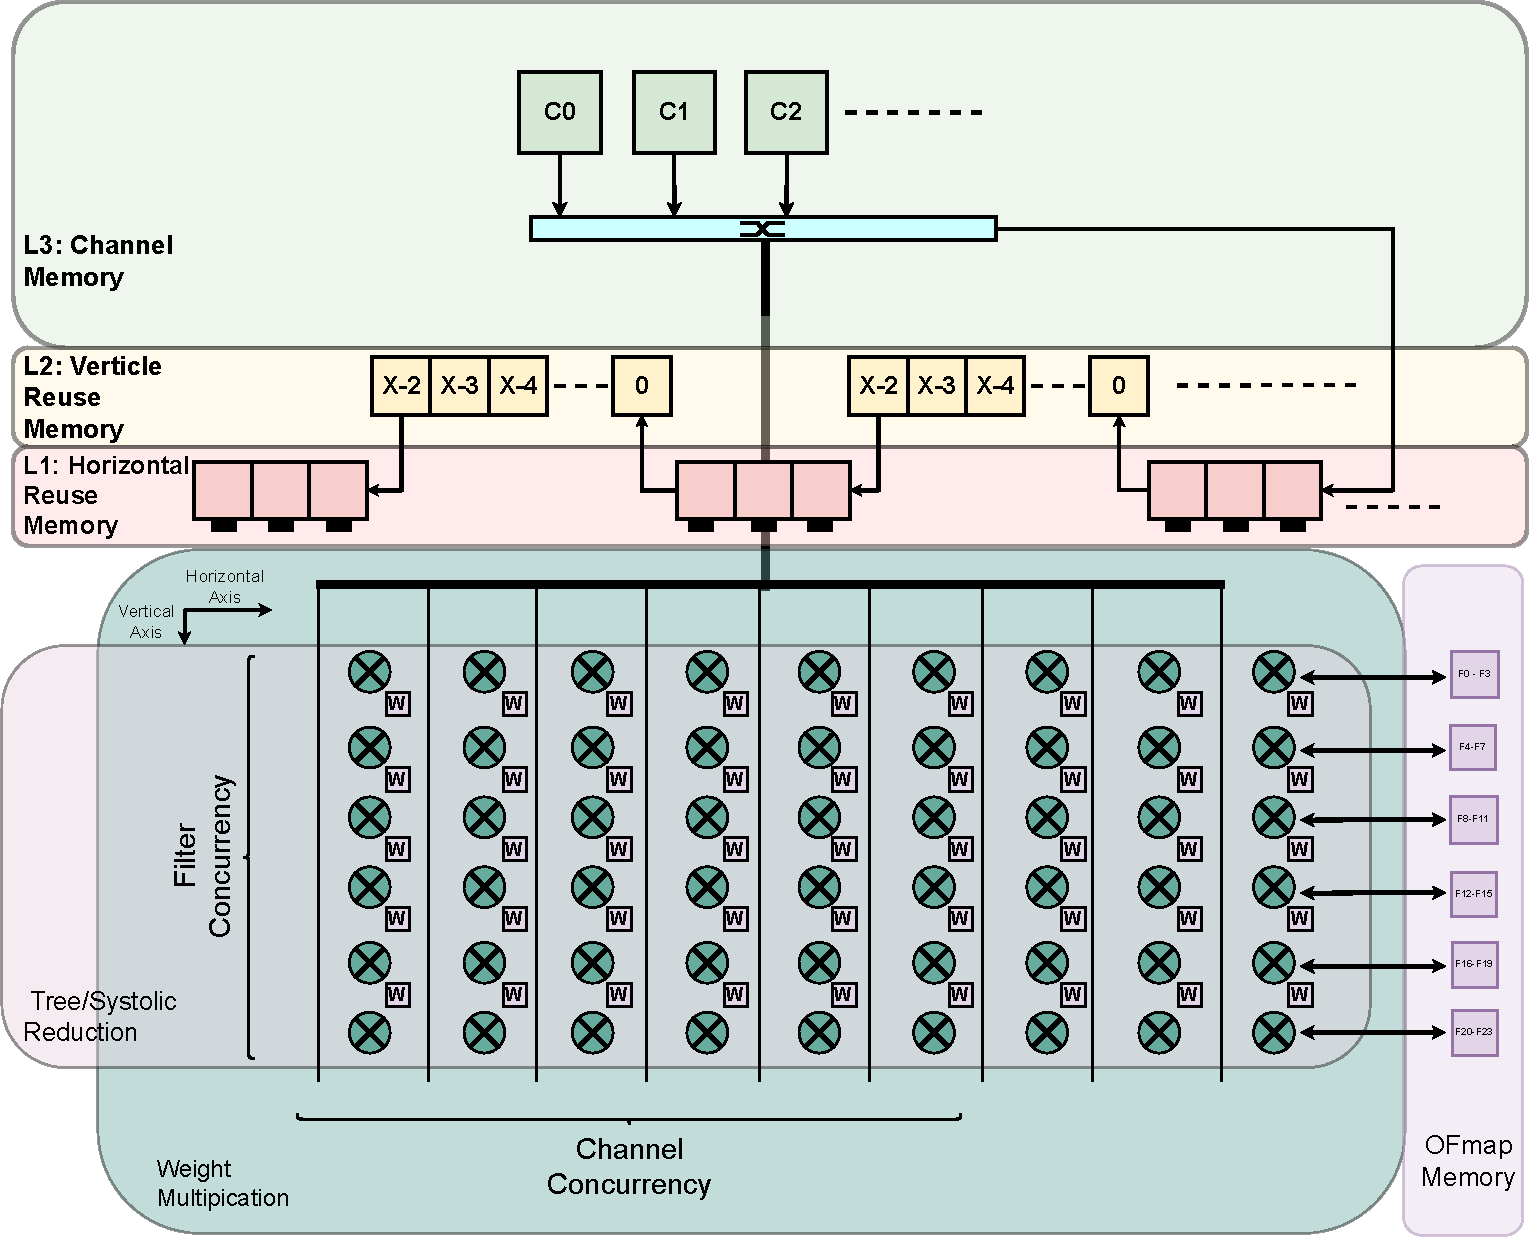
\includegraphics[scale=0.4]{fig/reuse_chain.pdf}
    \caption{Hardware template incorporating a reuse chain for reuse within an IFmap channel }
    \label{fig:reuse_chain}
\end{figure}


\subsection{Spatial Reuse Analysis}
\label{chap:dda:hw_dse:spatial_reuse_analysis}

So now we know the hierarchy needed to express X and Y reuse in IFmap. Applying
the unroll factors in the target loops in the dataflow will yield a loop
structure similar to the one in \ref{lst:conv_loops_unrolled_fully}. Using the
convention established in \ref{chap:hw_dse:temporal_analysis}, each
\ac{MAC} statement in the unrolled loop body has an associated j index. In the
loop body there exists duplicate memory accesses across individual \ac{MAC}
spatial instances. Those duplicate accesses are highlighted in
\autoref{lst:conv_loops_unrolled_fully} and they are the origin of spatial reuse
in the dataflow. IFmaps exhibit spatial reuse with multicast communication w.r.t
to filter loops. OFmap exhibit spatial reuse with reduction communication
w.r.t to channel loops. Weights exhibit no spatial reuse 
 
\clearpage
\begin{lstlisting}[language=C, caption=Spatial reuse in fully unrolled kernel loops, label={lst:conv_loops_unrolled_fully}]
for(int f = 0; f < F; f+=F_T) // Filter loop
    for(int c = 0; c < C; c+=C_T) // Channel loop
        for (int y = 0; y < Y; y++) // FeatureMap Height
            for(int x = 0; x < X; x++) // FeatureMap Width
            {
                %\colorbox{green}{O[f+0][y][x]}% += W[f+0][c+0][0][0] * \ 
                                    %\colorbox{yellow}{I[c+0][y+0][x+0]}%; // j=0
                %\colorbox{green}{O[f+0][y][x]}% += W[f+0][c+0][0][1] * \
                                    %\colorbox{yellow}{I[c+0][y+0][x+1]}%; // j=1
                %\colorbox{green}{O[f+0][y][x]}% += W[f+0][c+0][0][2] * \
                                    I[c+0][y+0][x+2];  // j=2
                %\colorbox{green}{O[f+0][y][x]}% += W[f+0][c+0][1][0] * \ 
                                    I[c+0][y+1][x+2];  // j=3
                ...
                %\colorbox{red}{O[f+1][y][x]}% += W[f+1][c+0][0][0] * \
                                    %\colorbox{yellow}{I[c+0][y+0][x+0]}%; // j=C_T*KY_T*KX_T
                %\colorbox{red}{O[f+1][y][x]}% += W[f+1][c+1][0][1] * \
                                    %\colorbox{yellow}{I[c+0][y+0][x+1]}%; // j=C_T*KY_T*KX_T+1
                ...
                O[f+F_T-1][y][x] += W[f+F_T-1][c+C_T-1][KY_T-1][KX_T-1] * \ 
                                        I[c][y+KY_T-1][x+KX_T-1]; 
                                                    // j=F_T*C_T*KY_T*KX_T-1
                                        
            }
\end{lstlisting}

Applying the taxonomy in \autoref{fig:hw_taxonomy} to data elements that are
spatially reused, IFmap channels that are spatially reused across unrolled
filter loops can be broadcast with a bus. The reuse chain discussed in
\autoref{chap:hw_dse:temporal_analysis} can be thought of as a
Store\&Forward scheme to deliver individual IFmap channel data elements to the
\ac{PE}s for reduction into OFmaps.Weights reused for channel iteration and are
discarded. They exhibit no spatial reuse, just temporal. Therefore they should
be kept in small on chip buffers, preferably close to the computation they are
used in. OFmap exhibit spatial reuse across concurrent channels as well as
temporal reuse across channel sets as discussed in
\autoref{chap:hw_dse:temporal_analysis}. A reduction tree as in
\autoref{fig:reduction_styles}.a or a systolic array reduce and fwd as in
\autoref{fig:reduction_styles}.b are both possible assuming no restrictions
arising from synthesis. Combining the reuse chain derived in
\autoref{chap:hw_dse:temporal_analysis} with the required systolic
delays yields a simplification to the L1 memory present in
\autoref{fig:reuse_chain}. This simplification is discussed in
\autoref{chap:hw_dse:simplifying_hierarchy}.


\begin{figure}
    \centering
    \subfigure[]{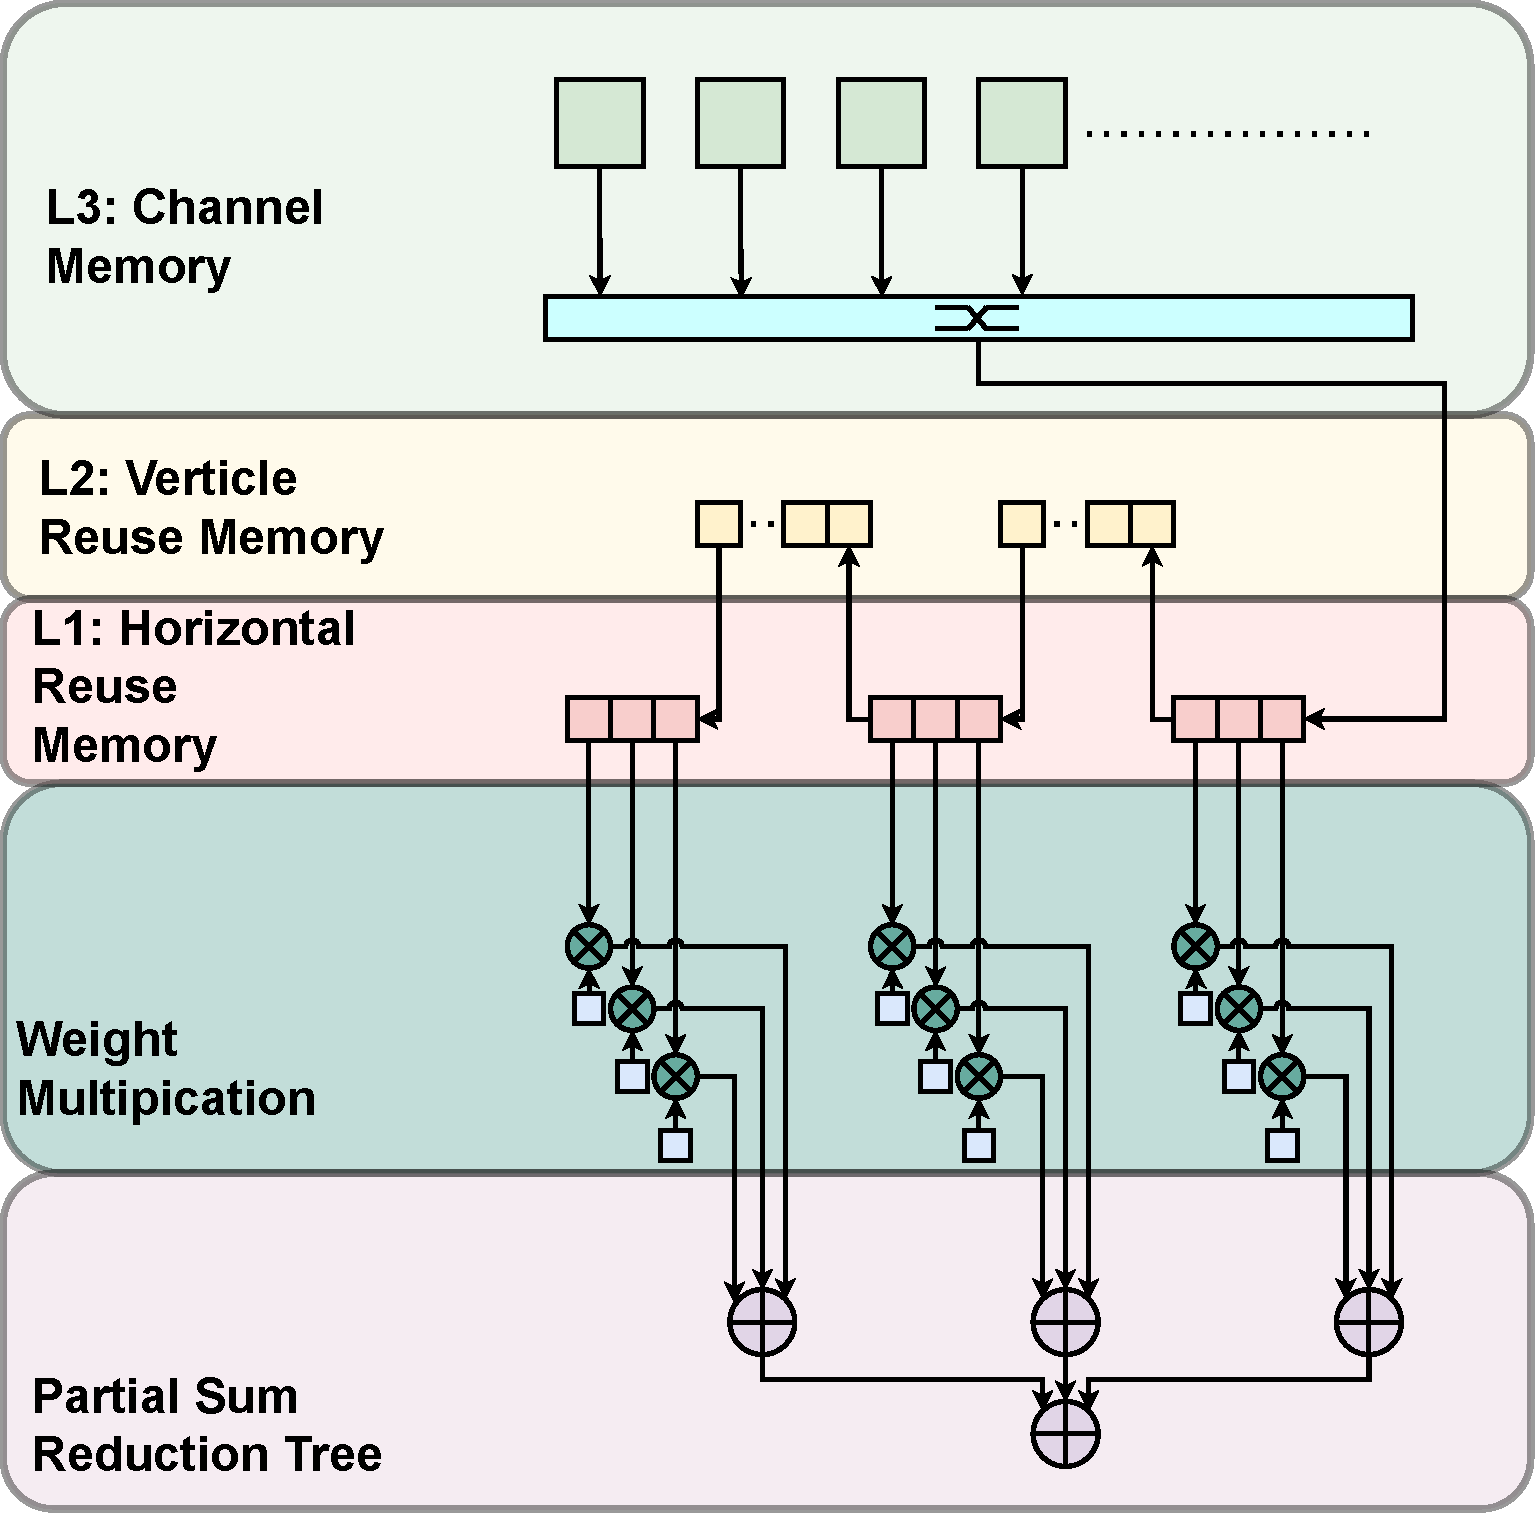
\includegraphics[width=0.5\textwidth]{fig/treeReduction.pdf}}
    \subfigure[]{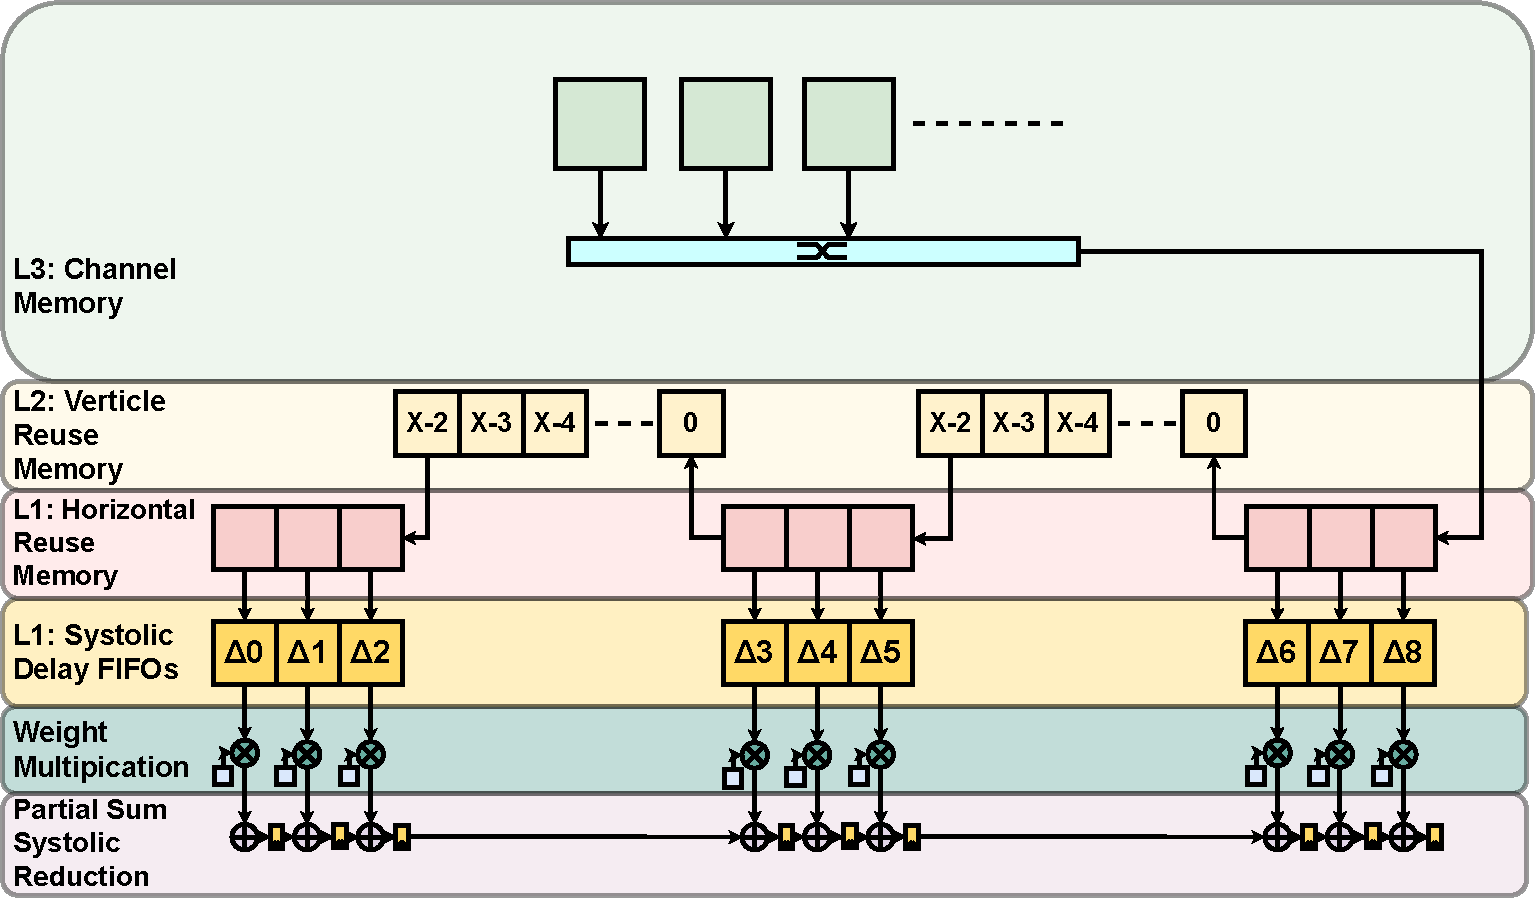
\includegraphics[width=0.7\textwidth]{fig/SystolicReduction.pdf}}
    \caption{Illustration of different partial sum reduction styles assuming kernel size is 3x3 (a) Tree Reduction (b) Systolic array reduction}
    \label{fig:reduction_styles}
\end{figure}

\subsection{Simplifying the memory hierarchy}
\label{chap:dda:hw_dse:simplifying_hierarchy}

\begin{figure}[]
    \centering
    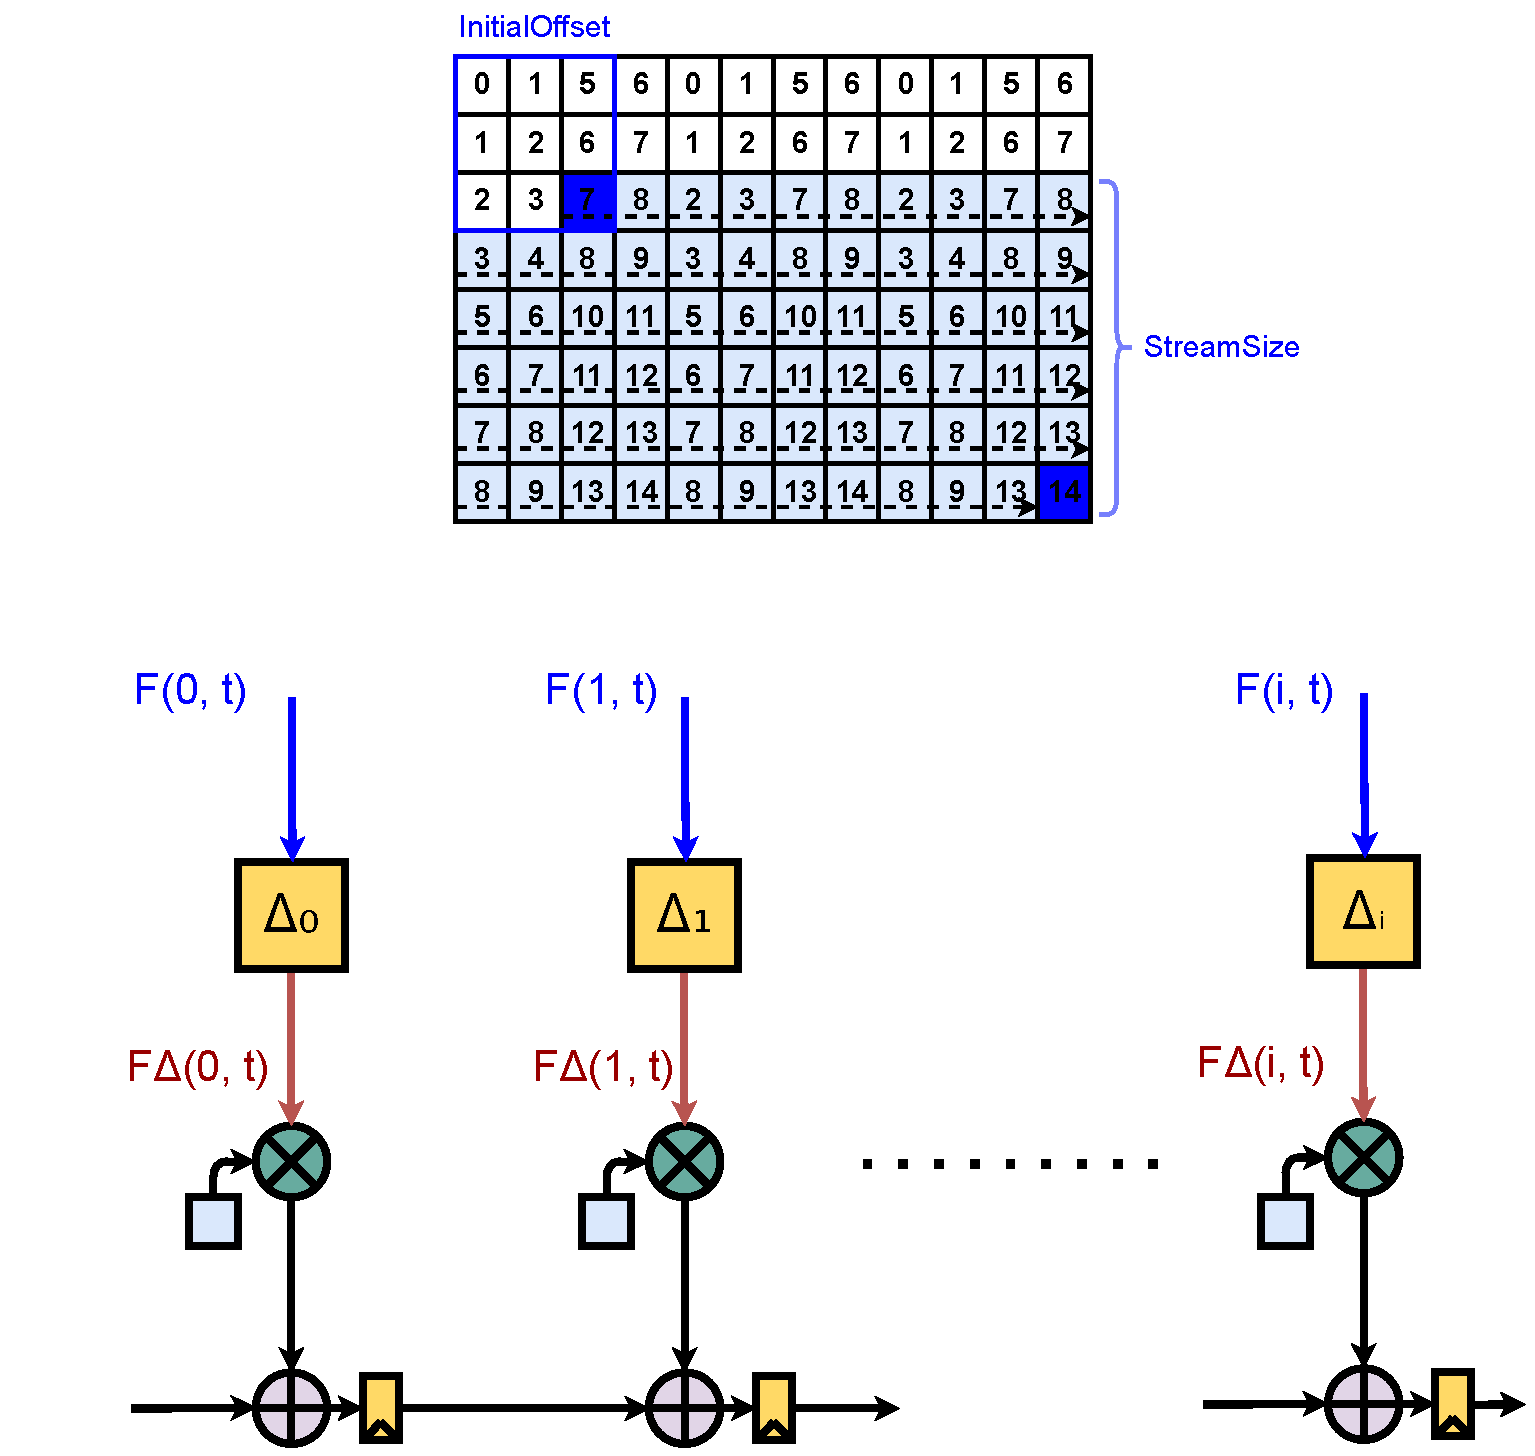
\includegraphics[scale=0.5]{fig/delayproof.pdf}
    \caption{Reinterpretation of IFmap memory hierarchy outputs as a stream function}
    \label{fig:delay_proof}
\end{figure}

We can reinterpret the accesses made by the IFmap memory hierarchy in
\autoref{fig:reuse_chain} as a stream function $F(i, t)$ whose output produces
element from an IFmap channel. The variable $i$ is the port index of IFmap
hierarchy and $t$ is the time in cycles since the beginning of the convolution
operation. A representation of this reinterpretation of the accesses made in the
IFmap memory hierarchy can be seen in \autoref{fig:delay_proof}. Since it's
always assumed that in direct mode kernel loops are unrolled fully the number of
ports into the IFmap memory hierarchy is always a multiple of $K^2$ where $K$ is
the size of the kernel being processed in direct mode. 

\begin{gather}
    IFmap \in R^{C\times n \times n} \xrightarrow{Reshape} IFmap \in R^{1\times Cn^2} \\
    Weight \in R^{F\times C\times K \times K} \\
    F(i, t)=    \begin{cases}
                    IFmap_{A(i, t)} & 0<=t < StreamSize \\
                    0 & else
                \end{cases} \\
    StreamSize = n(n-K)+(n-K) \\
    A(i, t) = InitialOffset(i) + t\\
\end{gather}

Each data element streamed from the IFmap depends on the an access function that
also takes the same variables $i$ and $t$. Depending on the port index $i$ the
access function for each port is composed on an initial offset in the IFmap and
the current cycle count. The number of cycles in which output from the IFmap
memory hierarchy can be produced is limited to the stream size of the IFmap
currently being processed. The stream size is a function of the IFmap dimensions
and the kernel Size. 

\begin{gather}
    InitialOffset = C_in^2+Y_in+X_i \\
    C_i = \lfloor \frac{\lfloor \frac{i}{K} \rfloor}{K} \rfloor \\
    Y_i = (\lfloor \frac{i}{K} \rfloor ) \bmod K\\
    X_i = i \bmod K = (i - \lfloor \frac{i}{K} \rfloor K)\\
\end{gather}

The initial offset function defines the initial index
offset in the IFmap the stream starts from for each port $i$. It can be
decomposed into three main offsets. A channel offset $C_i$, a row offset $Y_i$
and a column offset $X_i$. 

\begin{gather}
    F_\Delta(i, t) = \begin{cases}
    IFmap_{A_\Delta(i, t)} & \Delta_i<=t < \Delta_i+ StreamSize \\
    0 & else
    \end{cases} \\
    \Delta_i = i \\
    A_\Delta(i,t) = A(i, t) - \Delta_i\\
    % \hat{OFmap}(j) = \displaystyle\sum\limits_{i=0}^{ub(i)} A_\Delta(i, j+i)
\end{gather}

Under this new streaming based interpretation of the accesses in the IFmap
memory hierarchy, the delay elements in the systolic reduction scheme in
\autoref{fig:reduction_styles}.b are represented as time shifts in the stream
function $F(i,t)$. These time shifts are represented in the new delayed access
function $A_\Delta(i, t)$.

\begin{gather}
    A_\Delta(i,t) =  C_in^2+Y_in+(i - \lfloor \frac{i}{K} \rfloor K) + t- i\\
    A_\Delta(i,t) =  \lfloor \frac{\lfloor \frac{i}{K} \rfloor}{K} \rfloor^2+(\lfloor \frac{i}{K} \rfloor ) \bmod K + \underbrace{(- \lfloor \frac{i}{K} \rfloor K)}_{X'_i} + t\\
    % \hat{OFmap}(j) = \displaystyle\sum\limits_{i=0}^{ub(i)} A_\Delta(i, j+i)
\end{gather}

\begin{figure}[]
    \centering
    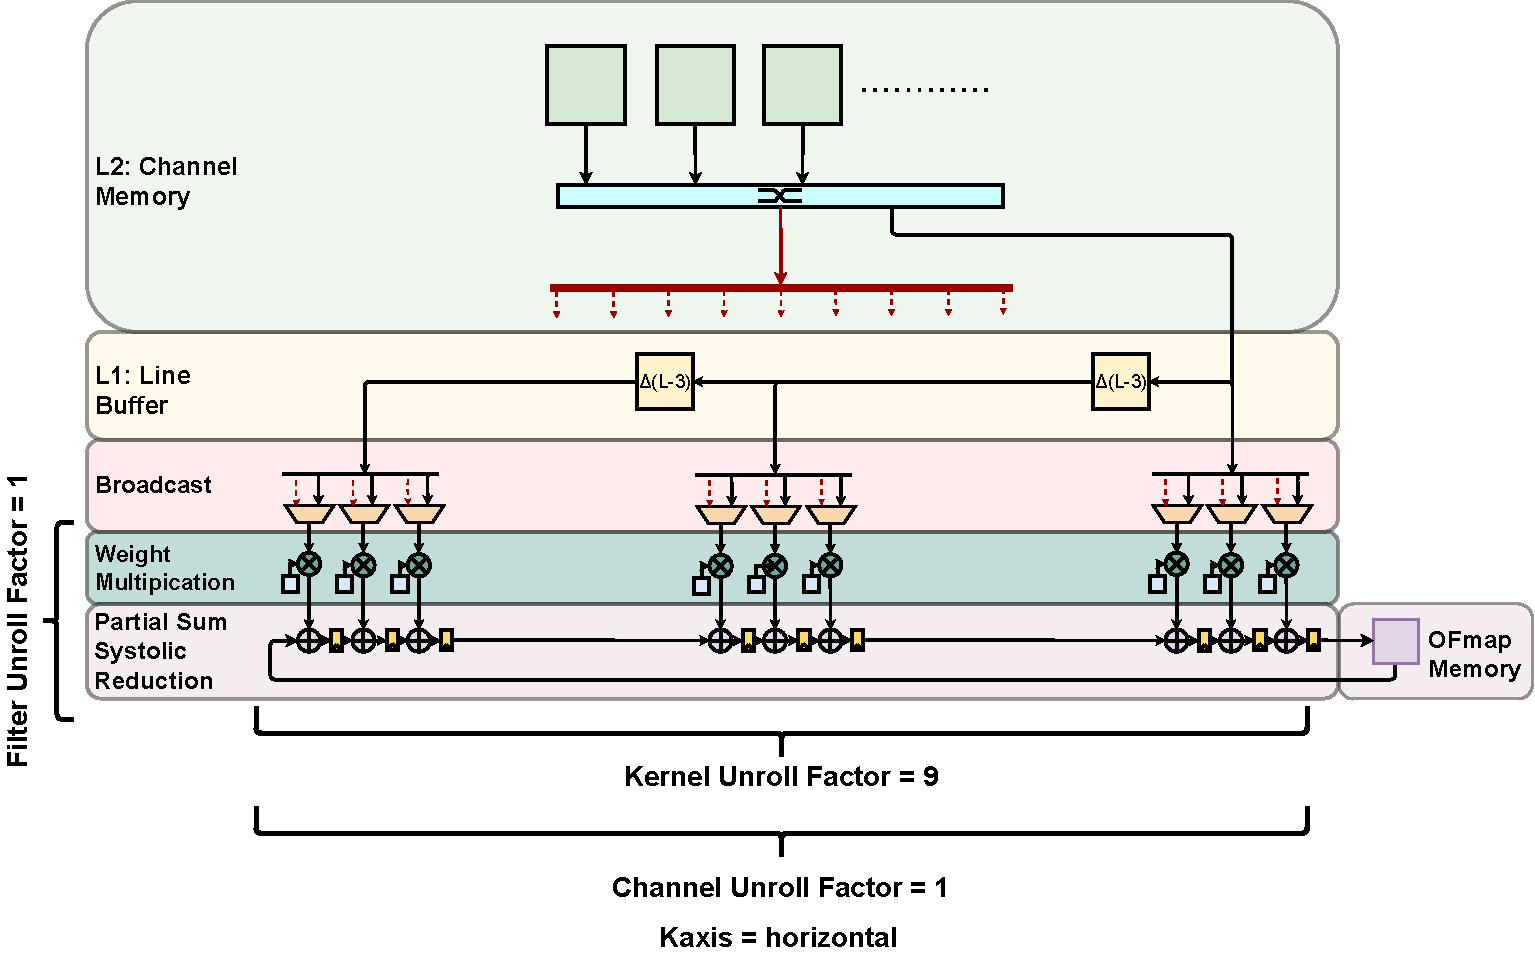
\includegraphics[scale=0.36]{fig/hybrid3x3Gemm.pdf}
    \caption{Using a systolic reduce and forward to calculate OFmaps}
    \label{fig:simplified_systolic_reduction}
\end{figure}

Substituting the InitialOffset function in $A_\Delta$  allows us to simplify the
column offset. This yields a new column offset $X'_i$. The final delayed access
function's initial offset becomes insensitive to changes in the port index $i$
that are not multiples of $K$. This allows us to remove the lowest layer memory
along with the systolic array delays in \autoref{fig:reuse_chain} and replace
both layers with just a series of broadcast buses that span consecutive $K$
groups of IFmap ports provided that we relax the start time constraints to the
$\lceil \frac{i}{K} \rceil$ for each group of ports $\lfloor \frac{i}{K}
\rfloor$. Delays in accessing IFmap data elements accross $K$ groups of ports
as well as accross $K^2$ groups of ports accessing different channels still
remain. This simplifying the hierarchy by removing the systolic delays thus still
requiring complex delayed reads from the IFmap hierarchy which necessitates smart
SRAMS whose access times can be programmed. A discussion of these smart memories
is presented in \autoref{chap:acc_sched:primitives:da-sram}. The final
hardware implementation with the added IFmap memory hierarchy optimization
discussed in this section is given in
\autoref{fig:simplified_systolic_reduction}.
\autoref{fig:simplified_systolic_reduction} shows the broadcast busses for every
group of 3 processing engines as well as the 1x1 vertical broadcast busses
highlighted in red. 

\section{HERO: A Hybrid GEMM and Direct Conv. Accelerator}
\label{chap:dda:hw_dse:final}

TEMPO's analytical model is hardware implementation agnostic
Tempo optimizes utilization given a library of networks + a pe budget
TEMPO reports average utilization, latency, and access count 
statistics
Then move on hero-t-sim to cycle accurate simulation results
Show performance for some popular networks

\begin{figure}[ht]
    \centering
    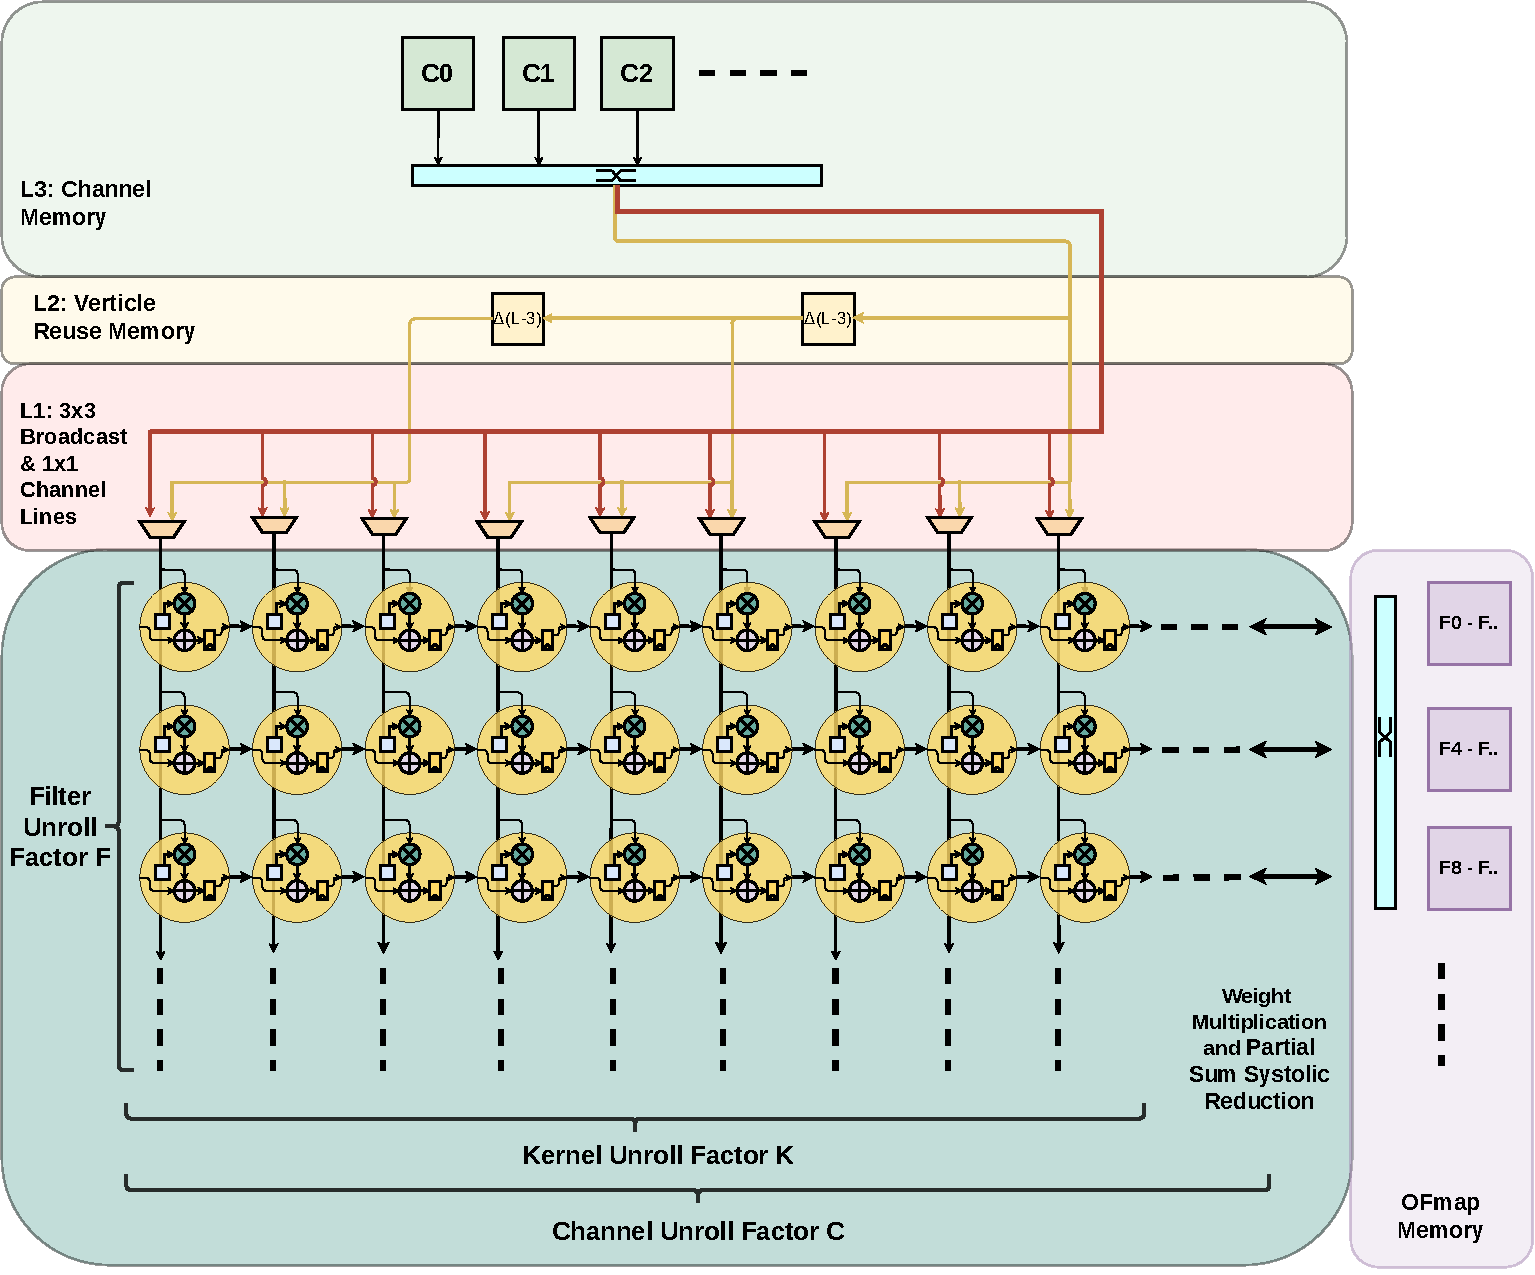
\includegraphics[scale=0.58]{fig/hero-t-horizontal.pdf}
    \caption{Hardware Implementation Taxonomy adapted from \cite{maestro}}
    \label{fig:hw_taxonomy}
\end{figure}

\begin{figure}[ht]
    \centering
    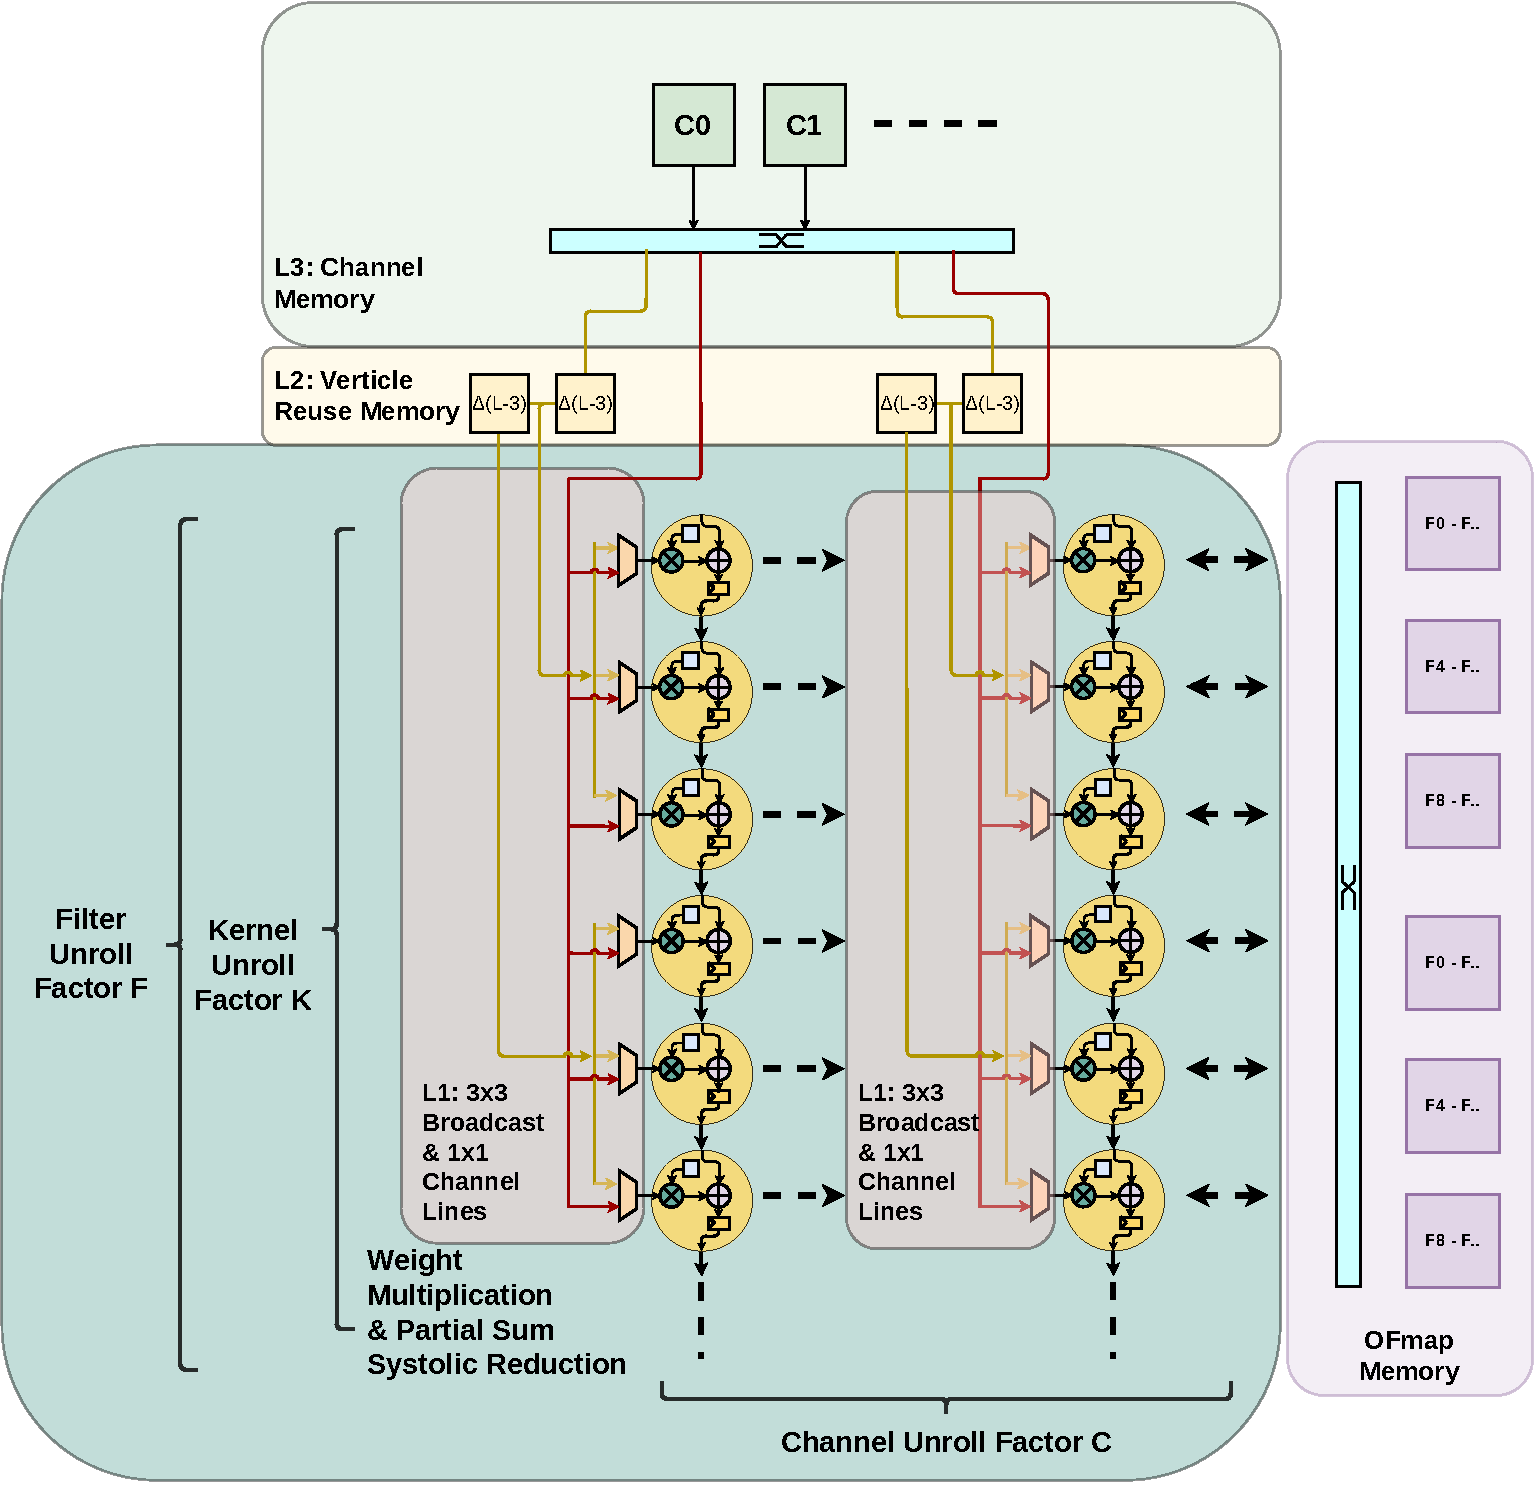
\includegraphics[scale=0.58]{fig/hero-t-verticle.pdf}
    \caption{Hardware Implementation Taxonomy adapted from \cite{maestro}}
    \label{fig:hw_taxonomy}
\end{figure}


